\documentclass[a4paper, 12pt]{article}

\usepackage{graphicx}
\usepackage[font=small, labelfont=bf, labelsep=colon]{caption}
\usepackage{amsmath, amssymb}
\usepackage{float}
\usepackage{textcomp}
\usepackage{siunitx}
\usepackage[dvipsnames]{xcolor}
\usepackage{titling} % To allow to use \matitle more than once
\usepackage{ctable}
\usepackage{multirow}
\usepackage[flushmargin, bottom]{footmisc} 
\usepackage{hyperref}
\usepackage{cleveref}


\hypersetup{
colorlinks = true,
linkcolor = {blue!80!black}
}

\graphicspath{{../../../Pictures/}}

%%%%%%%%%%%%%%%%%%%%%%%%%%%%%%%%%%%%%%%%%%%%%%%%%%%%%%%
% Layout parameters 
\setlength{\parindent}{0em}
\setlength{\parskip}{2ex}
\linespread{1.2}

\renewcommand{\floatpagefraction}{.99} % Minimum fraction of floats, in a page that has only floats. Only figures taking up more than that will get their own page. Default 0.5
\renewcommand{\topfraction}{0.99}  % Maximum fraction of page for floats at top. I.e.: floats taking up more than this will have no text below. Default: 0.7.
\renewcommand{\textfraction}{0.01} % Minimum fraction of page that must have text (otherwise, the page will only have float). Default: 0.2 

\addtolength{\textwidth}{2cm}
\addtolength{\hoffset}{-1cm}
\setlength{\topmargin}{-1cm}
\addtolength{\textheight}{1cm}

\setlength{\skip\footins}{6mm} % space between end of text and horizontal line of footnote
\setlength{\footnotesep}{5mm} % space between footnote line and first entry, and between consecutive entries of footnote



%%%%%%%%%%%%%%%%%%%%%%%%%%%%%%%%%%%%%%%%%%%%%%%%%%

%%%%%%%%%%%%%%%%%%%%%%%%
%%%%% NEW COMMANDS
%%%%%%%%%%%%%%%%%%%%%%%%

% Text commands
\newcommand{\spc}{1ex}
\newcommand{\eg}{\textit{e.g.}}
\newcommand{\ie}{\textit{i.e.}}

% Maths Commands
\newcommand{\R}{\mathbb{R}}
\newcommand{\bd}[1]{\boldsymbol{#1}}
\newcommand{\x}{\bd x}
\newcommand{\A}{{_{[A]}}}
\newcommand{\xA}{\bd{x^\A}}
\newcommand{\eps}{\varepsilon}
\newcommand{\Nr}{N_\text{regr}}
\newcommand{\E}{\mathbb{E}}
\newcommand{\Var}{\text{Var}}

\newcommand{\D}{\mathcal{D}}


\newcommand{\ya}{y^{(\alpha)}}
\newcommand{\yb}{y^{(\beta)}}
\newcommand{\ta}{\bd{\widetilde \alpha}}
\newcommand{\tb}{\bd{\widetilde \beta}}



%%%%%%%%%%%%%%%%%%%%%%%%%%%%%%%%%%%%%%%%%%%%%%%%%%%%%

\title{New Emulators for Monthly Gas Consumption}

\author{}
\date{}

\begin{document}

\maketitle
\vspace{-9ex}


This document is a concise summary of the construction and validation of the monthly gas consumption emulators. 
The 1000 design runs are divided into three sets:
\begin{itemize}
\item Training set (700 runs): used to train the emulators which predict the simulator's response on any other run;
\item Evaluation set (150 runs): used to choose the values of the emulator hyperparameters, by comparing the emulator's performance on the set with the know simulator's outputs;
\item Test set (150 runs): used to test the previously built emulators on a completely new set of runs not used in training and evaluation.
\end{itemize}
\autoref{Table_Var_names} lists the meaning and range of the 8 inputs which are varied from one simulation to the other.

\begin{table}
 \centering
 \renewcommand{\arraystretch}{1.4}
 \newcommand{\colsep}{4ex}
 \caption{Meaning and range of the eight parameters varied among the $n$ simulations of this work. {\it \footnotesize(Mohammad may provide more appropriate descriptions for the middle column.)}}
 \begin{tabular}{c<{\hspace{\colsep}}  c<{\hspace{\colsep}}  c}
\specialrule{.1em}{0em}{0.1em} 
 \textbf{Short Name} &  \textbf{Physical Meaning} & \textbf{Range} \\
 \specialrule{.05em}{.1em}{0.1em} 
 \specialrule{.05em}{0em}{0.2em} 
  $V_1$   &  Heating Setpoint               &  $[17.5, 20.5]$ $\si{\celsius}$        \\
  $V_2$   &  Boiler Efficiency              &  $[0.6, 0.75]$                         \\
  $V_3$   &  External wall thickness        &  $[4, 6.3]$ cm                         \\
  $V_4$   &  Roof quilt thickness           &  $[15, 21]$ cm                         \\
  $V_5$   &  Floor insulation thickness     &  $[4.5, 5.5]$ cm                       \\
  $V_6$   &  Infiltration rate              &  $[0.2, 0.95]$ ac/h                    \\
  $V_7$   &  DHW Consumption                &  $[6.15, 22] \!\times\! 10^{-6}$ litre/day \\
  $V_8$   &  Cooking                        &  $[1.05, 6.3]$ W/m$^2$                 \\
 \specialrule{.1em}{0.2em}{1em} 
 \end{tabular}
\label{Table_Var_names}
\end{table}

\section{Emulators' Training}
In order to emulate the monthly gas consumption, the range of each of the eight input variables $V_1, \dots, V_8$ has been linearly rescaled into $[-1,1]$.
Given the outputs $y_i$ of the 700 training runs for a given month, 
I have first built a linear regression model of $y_i$ as a function of (some of the) linear, quadratic and interaction terms of the $V_i$.
Hence, I have built an emulator of the linear regression residuals. Details of the two steps follow.

\subsubsection*{Linear Regression}
Let $\mathcal{R}$ be the set of all linear, quadratic and interaction terms of the 8 inputs $V_1, \dots, V_8$, all mutually orthogonal.
As it turns out, for all months, the set of the ``best'' 10 regressors in $\mathcal{R}$ (the set maximising the adjusted $R^2$) explains the data extremely well, 
with an adj-$R^2$ of about 0.999 in all cases. Given the excellent result, and to use an approach which is uniform among months and simple to explain,  
for each month I have built a linear regression model by selecting the best 10 regressors according to the above criterion. 
\emph{(previously, for May, I was using some 3rd-order terms to improve the linear model. Probably not worth it)}

\autoref{Table_Regressors} shows which 10 regressors have been selected for each month, the adjusted $R^2$ of the associated linear model, and the variance of the residuals.

\begin{table}
 \centering
 \renewcommand{\arraystretch}{1.4}
 \newcommand{\colsep}{3ex}
 \caption{For each of the nine months considered, from left to right: the set of covariates used to build the linear regression model, the adjusted $R^2$ of the model, the variance of the residuals.
 In the second column, the ``$\ast$'' symbol is used as shorthand notation to denote all linear and interaction terms, \eg\ $\,a \ast b \ast c = \{ a, b, c , ab, ac, bc \}$.}
 \begin{tabular}{c<{\hspace{\colsep}}  c<{\hspace{\colsep}}  c<{\hspace{\colsep}} c}
\specialrule{.1em}{0em}{0.1em} 
 \textbf{Month} &  \textbf{Regressors} & \textbf{Adj.~$R^2$} & \textbf{Resid.~Var.~$\sigma^2$}\\
 \specialrule{.05em}{.1em}{0.1em} 
 \specialrule{.05em}{0em}{0.2em} 
  Jan  &  $V_1 \!\ast\! V_2 \!\ast\! V_6, \,V_3,\, V_4,\,{V_2}^2,\, {V_6}^2$   & 0.9998   & 85.94\\
  Feb  &  $V_1 \!\ast\! V_2 \!\ast\! V_6, \,V_3,\, V_4,\,{V_2}^2,\, {V_6}^2$   & 0.9998  &  52.30\\
  Mar  &  $V_1 \!\ast\! V_2 \!\ast\! V_6, \,V_3,\, V_4,\,{V_2}^2,\, {V_6}^2$   & 0.9997  &  50.14\\
  Apr  &  $V_1 \!\ast\! V_2 \!\ast\! V_6, \,V_3,\, V_4,\,{V_2}^2,\, {V_6}^2$   & 0.9998  &  50.04\\  
  May  &  $V_1 \!\ast\! V_2 \!\ast\! V_6, \,V_3,\, V_8,\,{V_1}^2,\, {V_6}^2$   & 0.9989  & 206.45\\
  Sep  &  $V_1 \!\ast\! V_2 \!\ast\! V_6, \,V_3,\, V_4,\, V_8,\, {V_6}^2$         & 0.9994  &  0.91\\
  Oct  &  $V_1 \!\ast\! V_2 \!\ast\! V_6, \,V_3,\, V_4,\, V_8,\, {V_6}^2$         & 0.9996  &  24.40\\
  Nov  &  $V_1 \!\ast\! V_2 \!\ast\! V_6, \,V_3,\, V_4,\,{V_2}^2,\, {V_6}^2$   & 0.9998 &  57.35\\
  Dec  &  $V_1 \!\ast\! V_2 \!\ast\! V_6, \,V_3,\, V_4,\,{V_2}^2,\, {V_6}^2$   & 0.9998  &  68.77\\
 \specialrule{.1em}{0.2em}{1em} 
 \end{tabular}
\label{Table_Regressors}
\end{table}


\subsubsection*{Bayes Linear Emulators of Residuals}
In order to build an emulator of the residuals, choices about the following are to be made: active inputs, correlation lengths, prior emulator variance and nugget variance.

To choose these, for each month, I have followed the general procedure which I highlight below. In particular, the procedure to choose active inputs and correlation lengths has involved visual assessment of the emulator's performance on the evaluation set, by plotting the standardised residuals for the runs of this set. \autoref{Validation} will provide details and graphs on this. 

\begin{itemize}
\item {\bf Active Inputs}: To identify which inputs were significant in explaining the residuals, I have looked at the best selection of second- (and sometimes third-) order terms in a linear regression model. 
Terms which would appear alone with a significant $t$-value ($t>8$) would be included as an active input; the inclusion of terms appearing only in interaction with other terms or with a low $t$-value would instead be considered case by case, according to the emulator performance on the evaluation set.
\item {\bf Correlation lengths}: Once the active inputs have been chosen, I have used the same correlation length for all of them. The correlation length has been chosen by assessing the emulator's performance on the validation set, also accounting for the number of active inputs used
(to attain a similar level of correlation across the space, higher correlation lengths are needed if more active inputs are used).
\item {\bf Prior Variances}: The cumulative prior variance (the one of the second-order stochastic process over which we make specifications, plus the one of the ``nugget'' process) has been imposed to be the variance of the residuals which are being fitted. This overall variance has been split into the two components in the proportions of $95\%$ and $5\%$, respectively.
\end{itemize}

\autoref{Table_Emulator_Specifications} shows the choices of the above quantities for the nine months of interest.
\autoref{Fig_Correlation} instead gives an idea of the level of correlation across the input space induced by the above choices. Specifically, named $P$ the point at the centre of the hypercube with edges $[-1,1]$, the figure shows histograms of the correlation between the point $P$ and 2 million uniformly distributed points in the hypercube.



\begin{table}
 \centering
 \renewcommand{\arraystretch}{1.4}
 \newcommand{\colsep}{3ex}
 \caption{For each of the nine months considered, the table below shows which active inputs have been chosen and the value of the correlation length (same for all active inputs).}
 \begin{tabular}{c<{\hspace{\colsep}}  c<{\hspace{\colsep}}  c<{\hspace{\colsep}} c}
\specialrule{.1em}{0em}{0.1em} 
 \textbf{Month} &  \textbf{Active Inputs} & \textbf{Corr.~Length}\\
 \specialrule{.05em}{.1em}{0.1em} 
 \specialrule{.05em}{0em}{0.2em} 
  Jan  &  $V_1, \,V_2, \,V_3, \,V_6, \,V_8$               &  0.8\\
  Feb  &  $V_1, \,V_2, \,V_3, \,V_7, \,V_8$               &  0.65\\
  Mar  &  $V_1, \,V_2, \,V_3, \,V_6, \,V_7, \,V_8$   &  1.3\\
  Apr  &  $V_1, \,V_2, \,V_3, \,V_6, \,V_8$              &  1.0\\  
  May  &  $V_1, \,V_2, \,V_3, \,V_4, \,V_6, \,V_8$  &  1.0\\
  Sep  &  $V_1, \,V_2, \,V_3, \,V_6, \,V_7, \,V_8$   &  1.2\\
  Oct  &  $V_1, \,V_2, \,V_3, \,V_6, \,V_7, \,V_8$   &  1.4\\
  Nov  & $V_1, \,V_2, \,V_3, \,V_6, \,V_7, \,V_8$   & 1.2\\
  Dec  &  $V_1, \,V_2, \,V_3, \,V_6, \,V_7, \,V_8$  & 1.3\\
 \specialrule{.1em}{0.2em}{1em} 
 \end{tabular}
\label{Table_Emulator_Specifications}
\end{table}


\newcommand{\scale}{12.7em}
\begin{figure}
\centering
 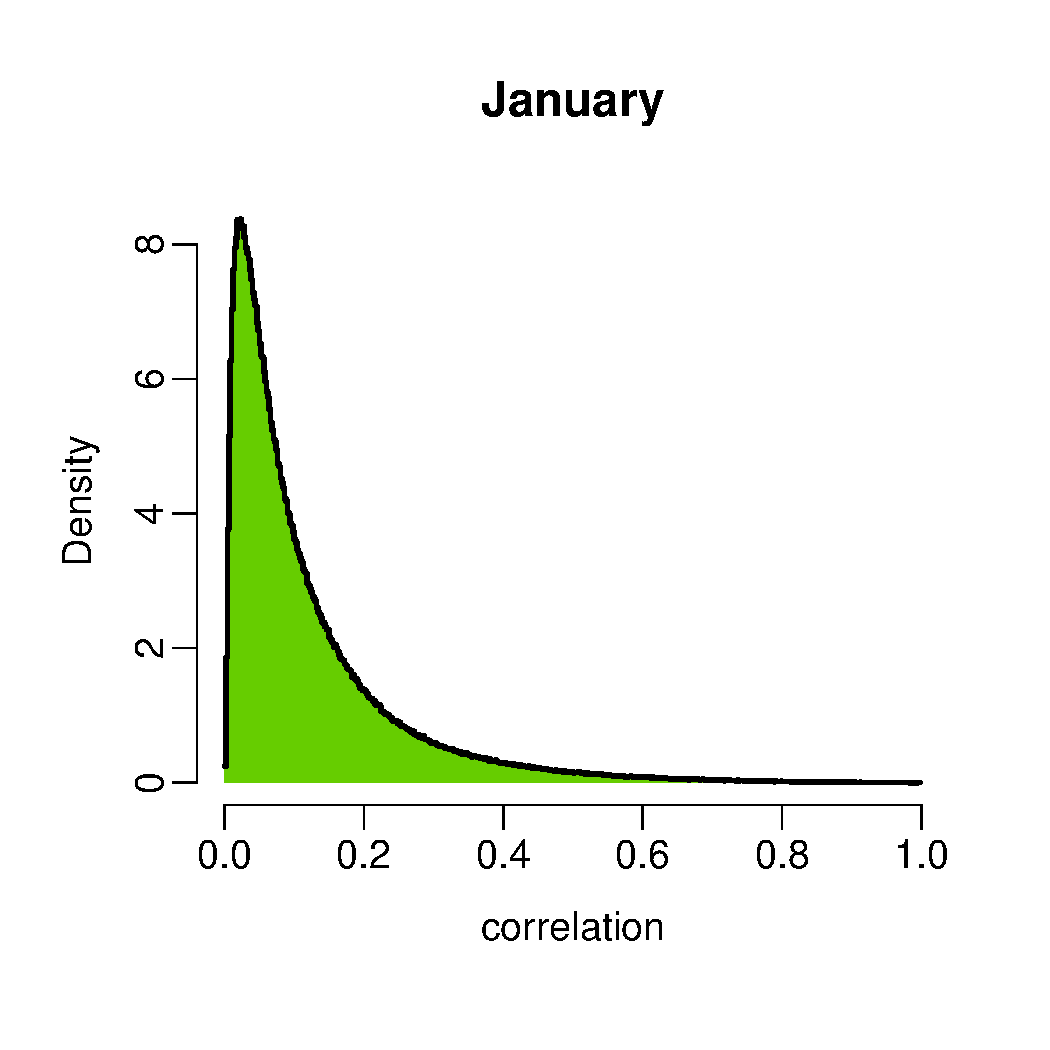
\includegraphics[width=\scale]{Validation_Plots/Correlation/Correlation_01_Jan}\hspace{-1ex}
 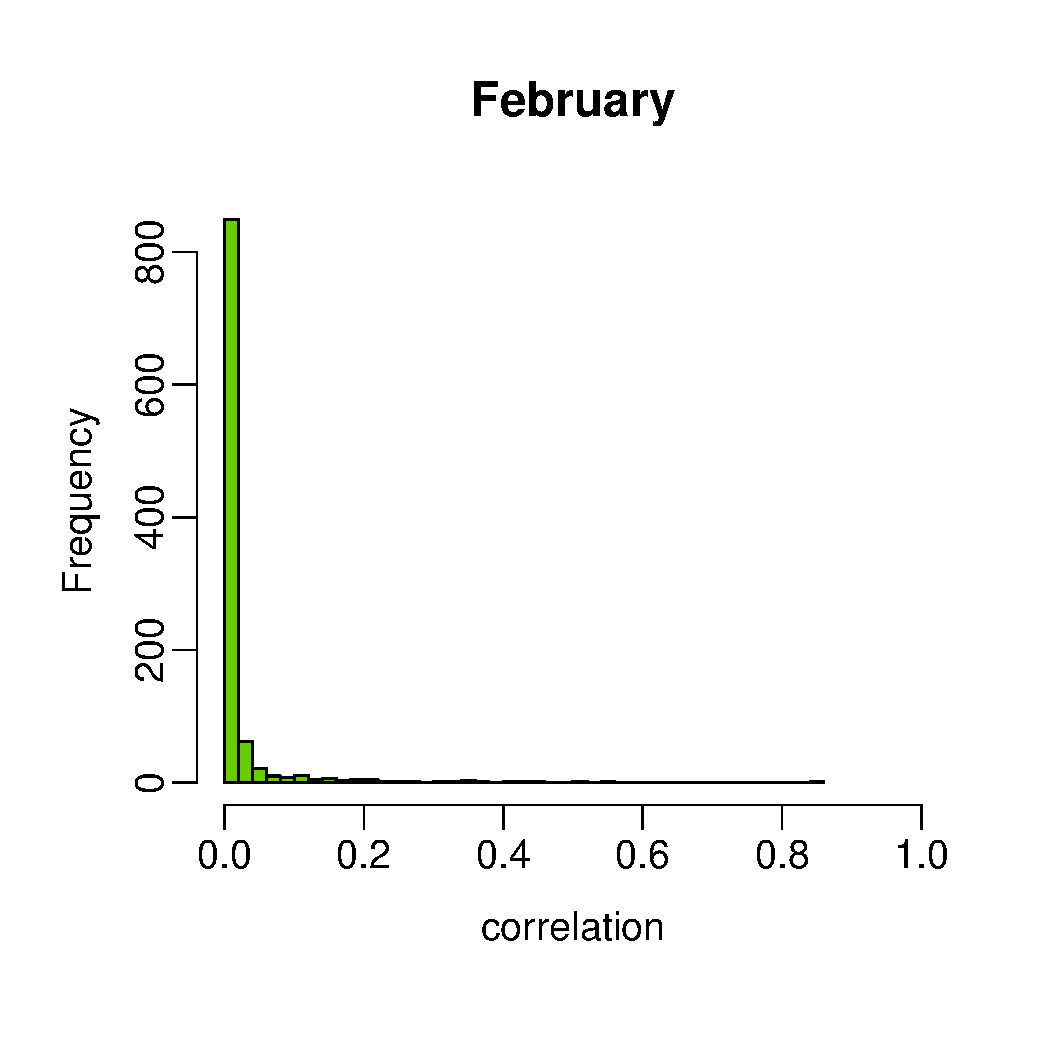
\includegraphics[width=\scale]{Validation_Plots/Correlation/Correlation_02_Feb}\hspace{-1ex}
 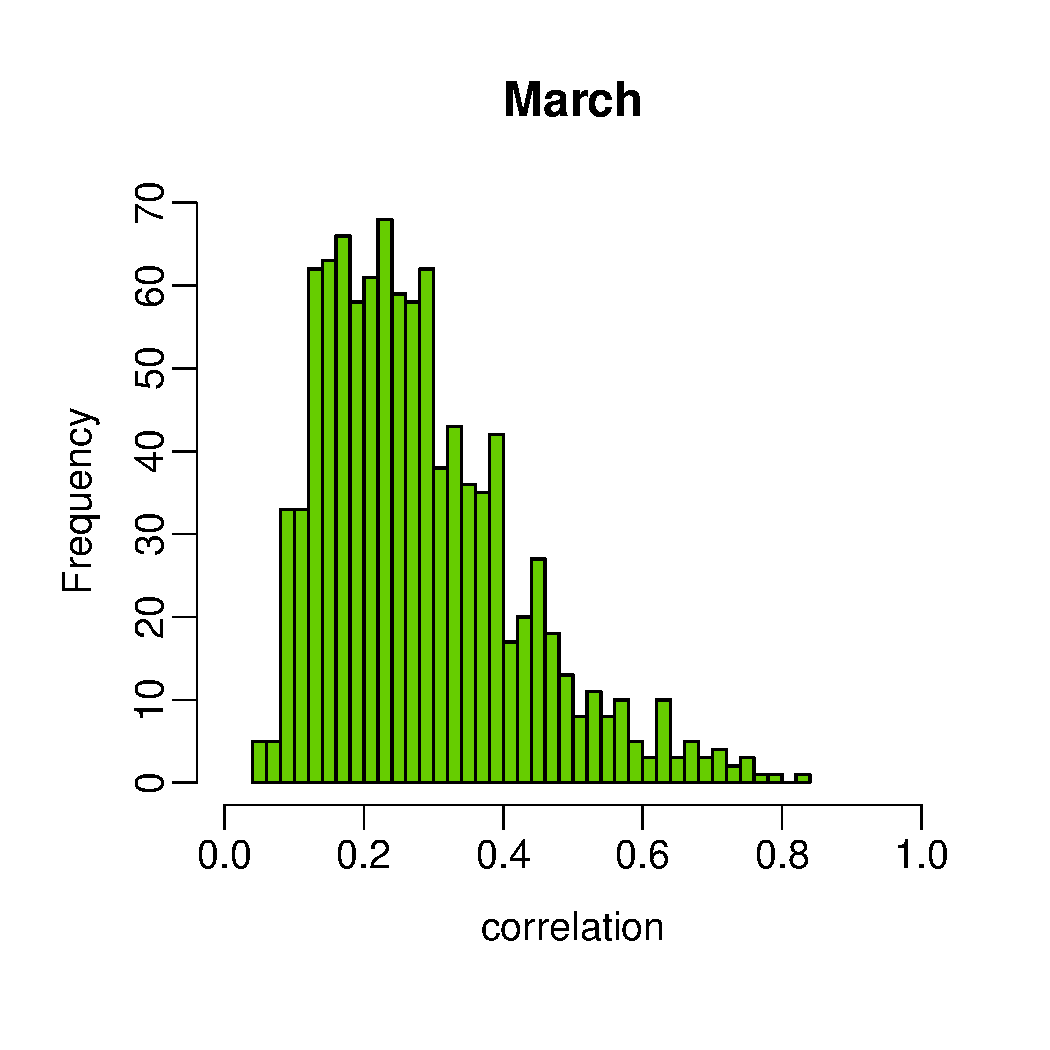
\includegraphics[width=\scale]{Validation_Plots/Correlation/Correlation_03_Mar}\\[-3ex]
 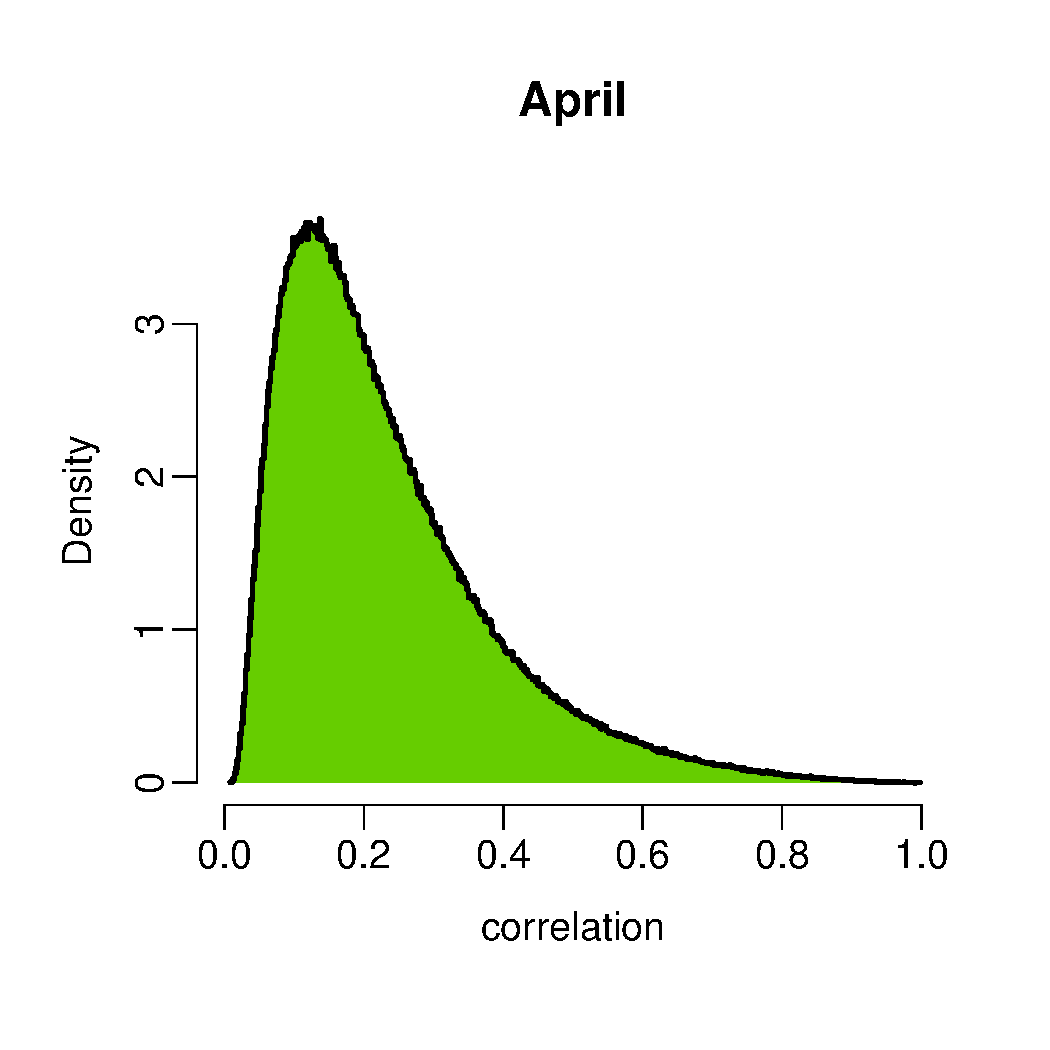
\includegraphics[width=\scale]{Validation_Plots/Correlation/Correlation_04_Apr}\hspace{-1ex}
 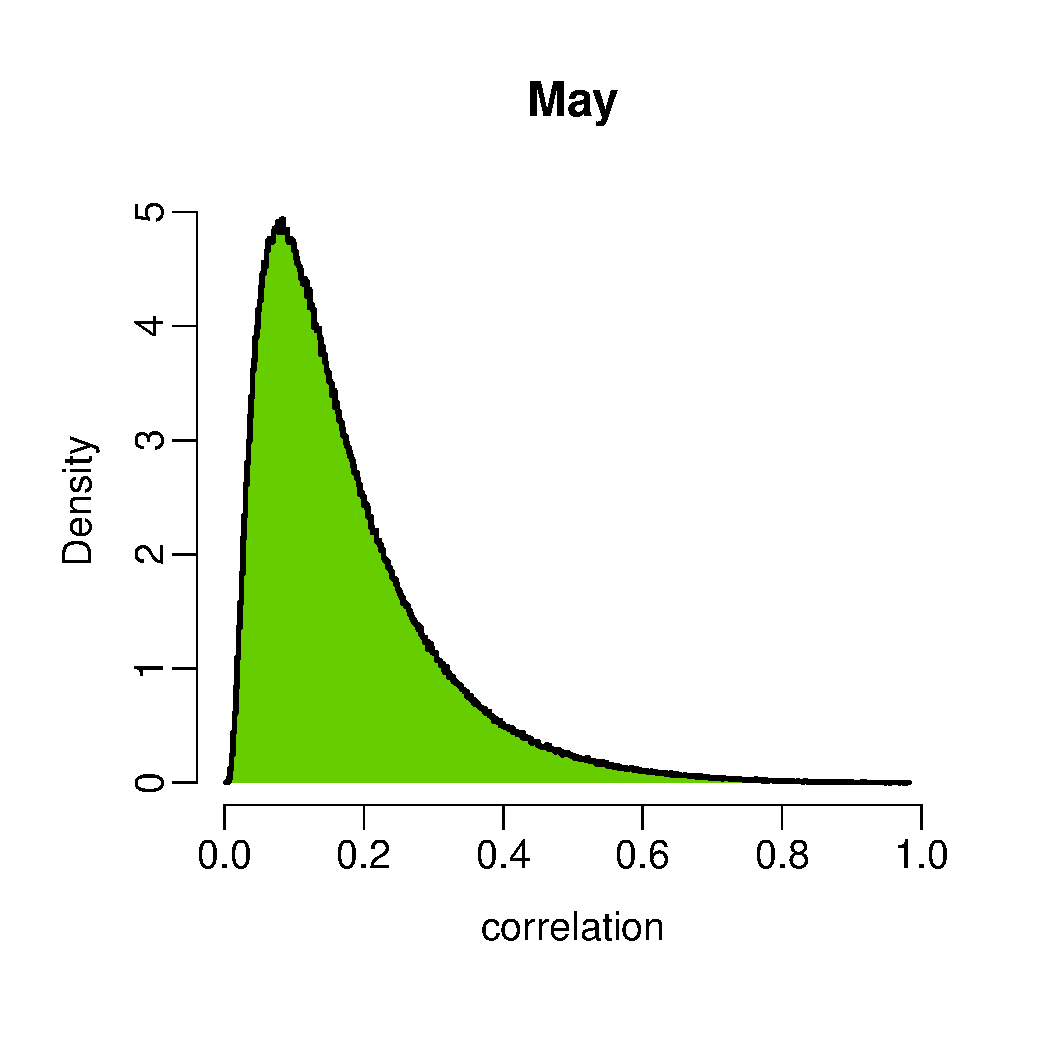
\includegraphics[width=\scale]{Validation_Plots/Correlation/Correlation_05_May}\hspace{-1ex}
 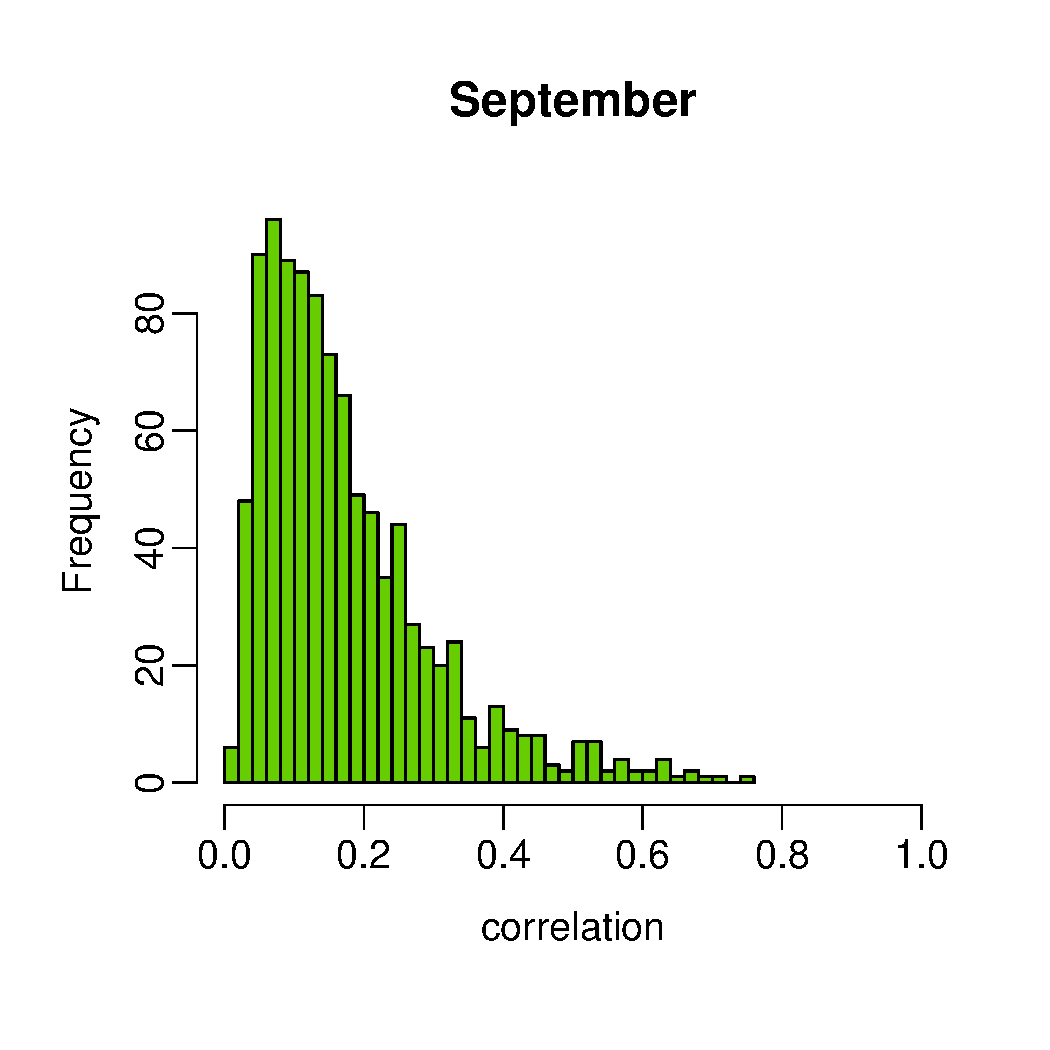
\includegraphics[width=\scale]{Validation_Plots/Correlation/Correlation_09_Sep}\\[-3ex]
 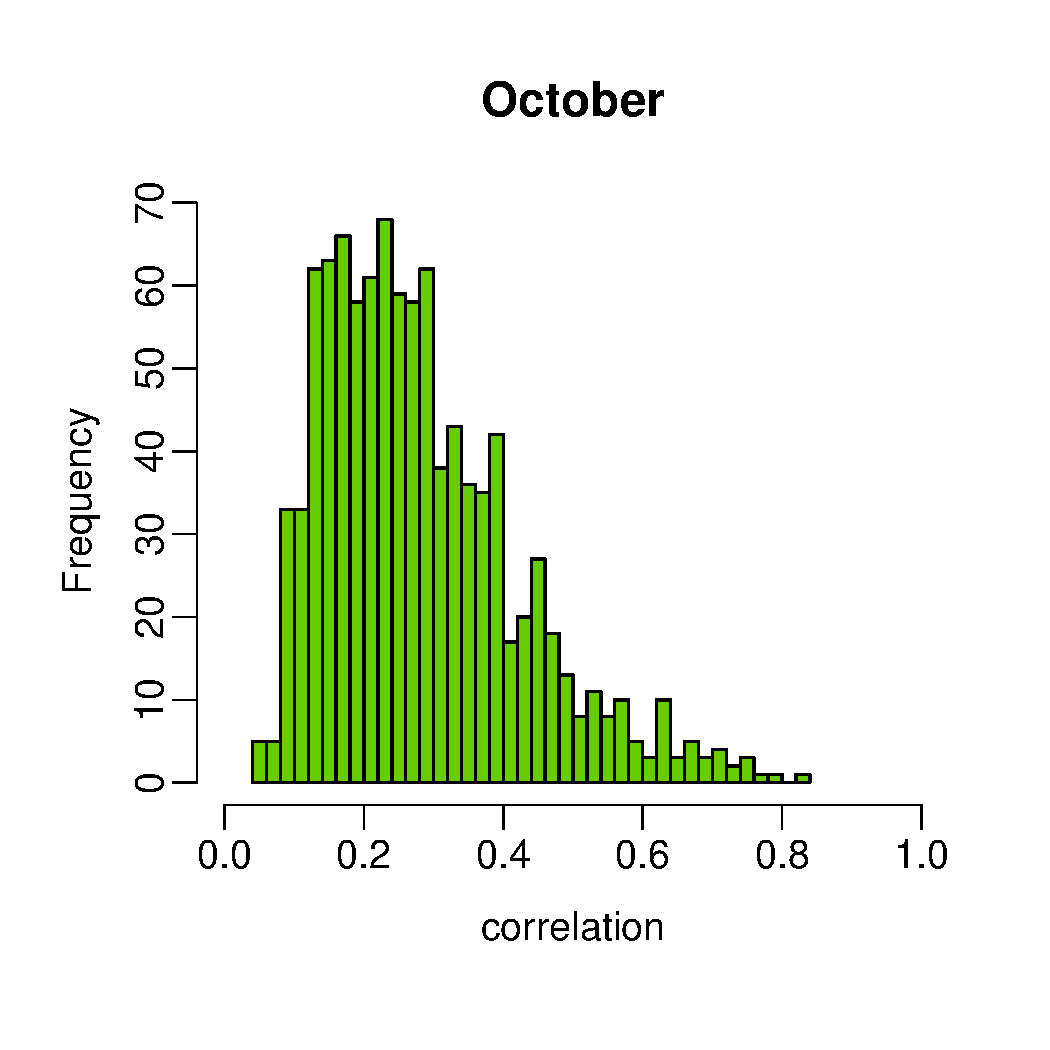
\includegraphics[width=\scale]{Validation_Plots/Correlation/Correlation_10_Oct}\hspace{-1ex}
 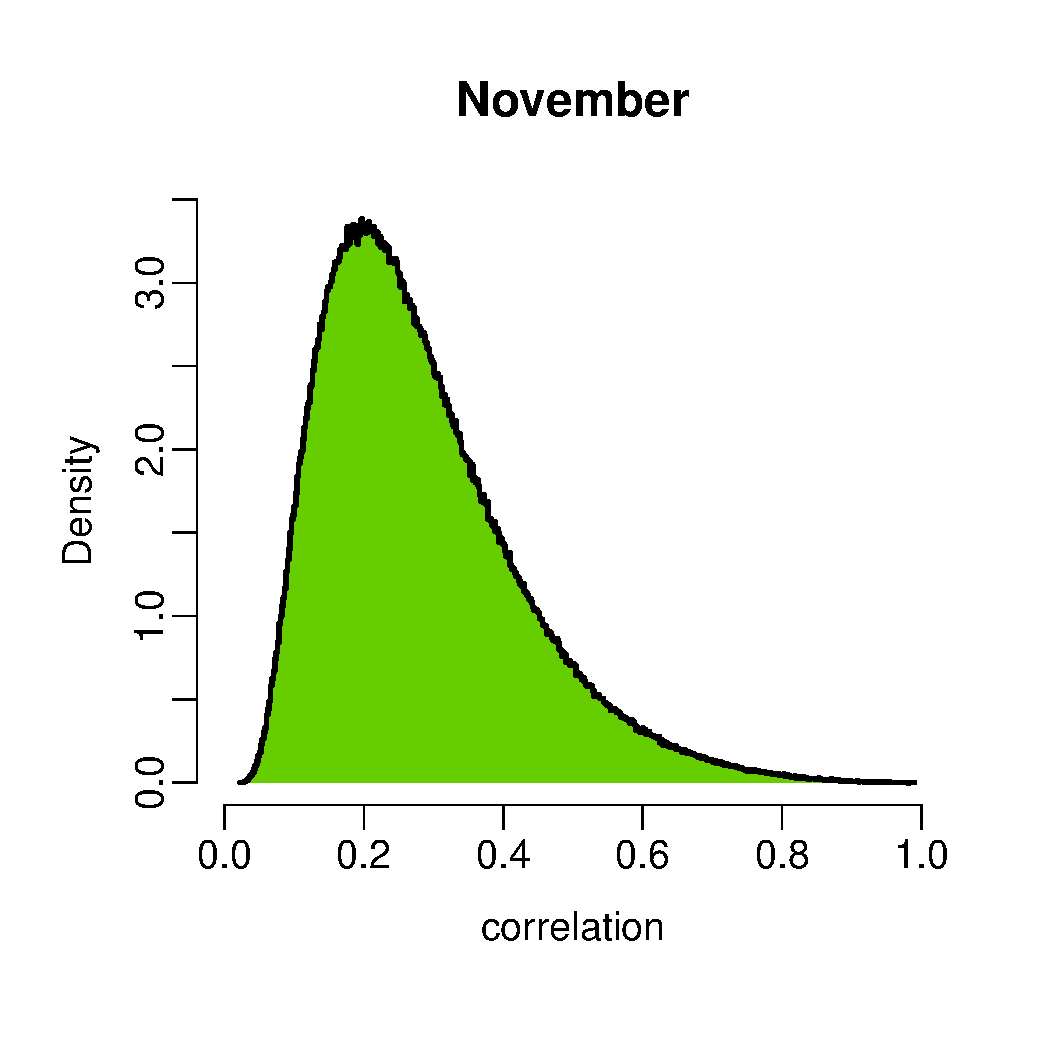
\includegraphics[width=\scale]{Validation_Plots/Correlation/Correlation_11_Nov}\hspace{-1ex}
 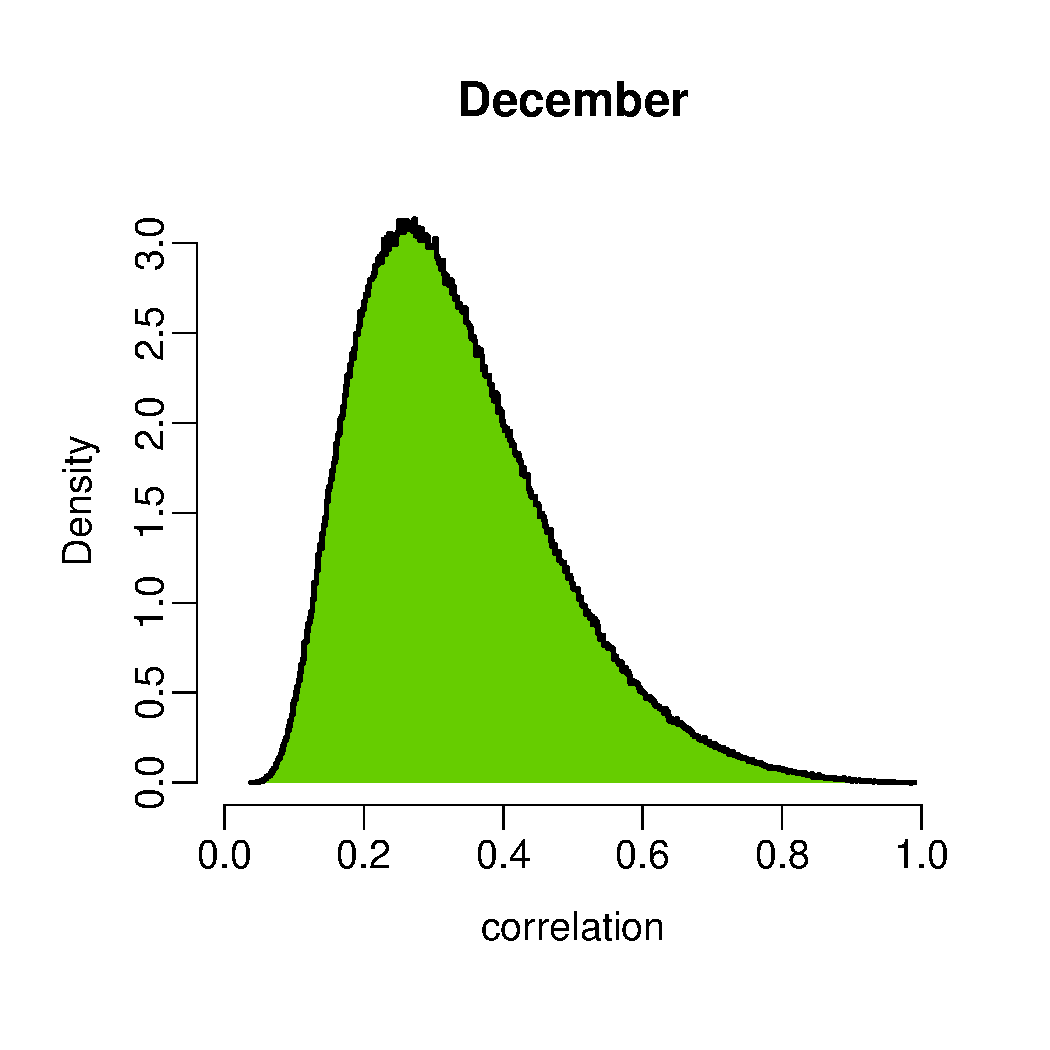
\includegraphics[width=\scale]{Validation_Plots/Correlation/Correlation_12_Dec}
 \caption{Histograms of the correlations between the point at the center of the hypercube $[-1,1]^N$ (where, for each month, $N$ is the number of active inputs) and $2\times 10^6$ uniformly distributed points in the hypercube.}
 \label{Fig_Correlation}
\end{figure}



\section{Emulators' Validation and Exploration}\label{Validation}
This section concerns the validation of the previously built emulators. Choices of the active inputs and hyperparameters have been made based on the performance of the emulators on an evaluation set consisting of 150 observations not used in training. The emulators built this way have then been used to predict the simulated values of a completely new test set, consisting of additional 150 observations. 

\renewcommand{\scale}{12.7em}
\begin{figure}
\centering

 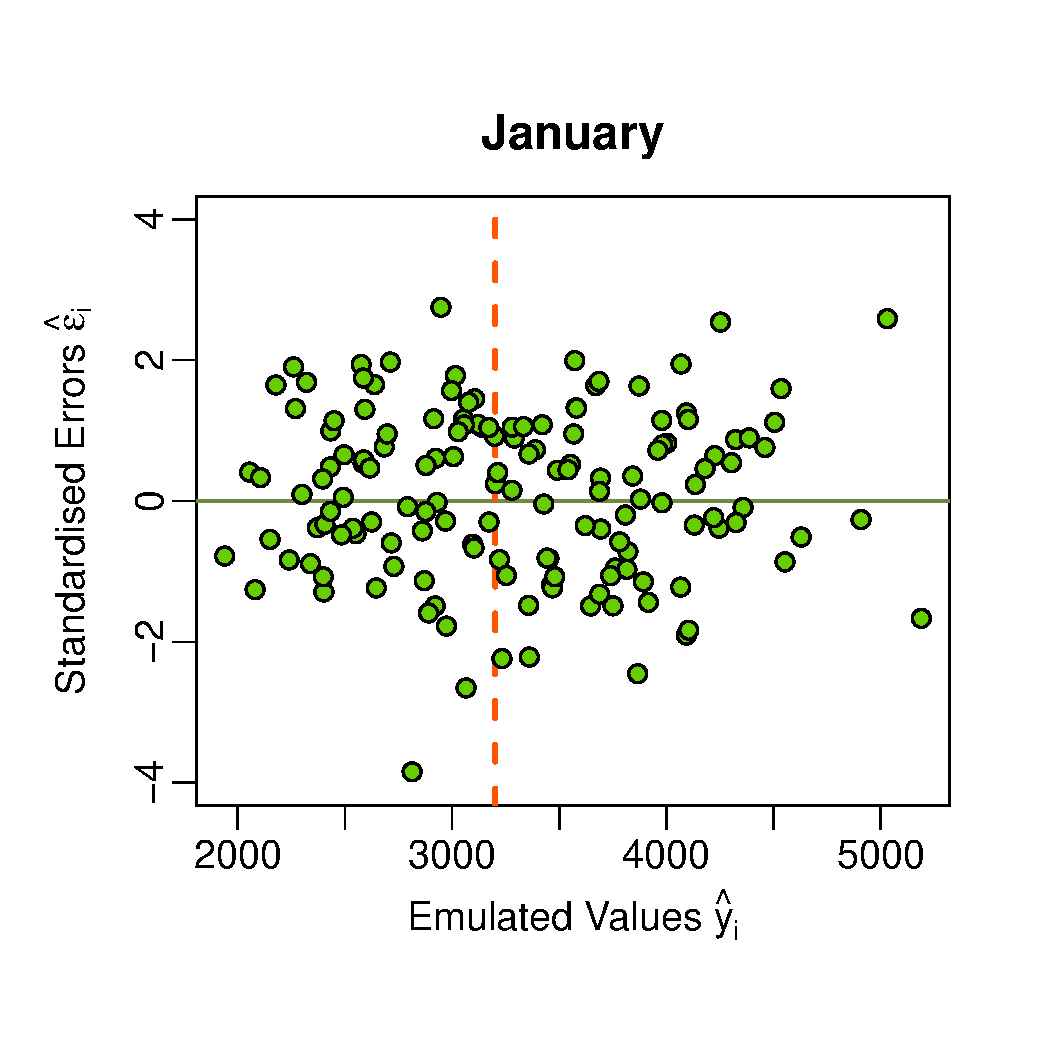
\includegraphics[width=\scale]{Validation_Plots/Evaluation_Set/Evaluation_Scatter_01_Jan}\hspace{-1ex}
 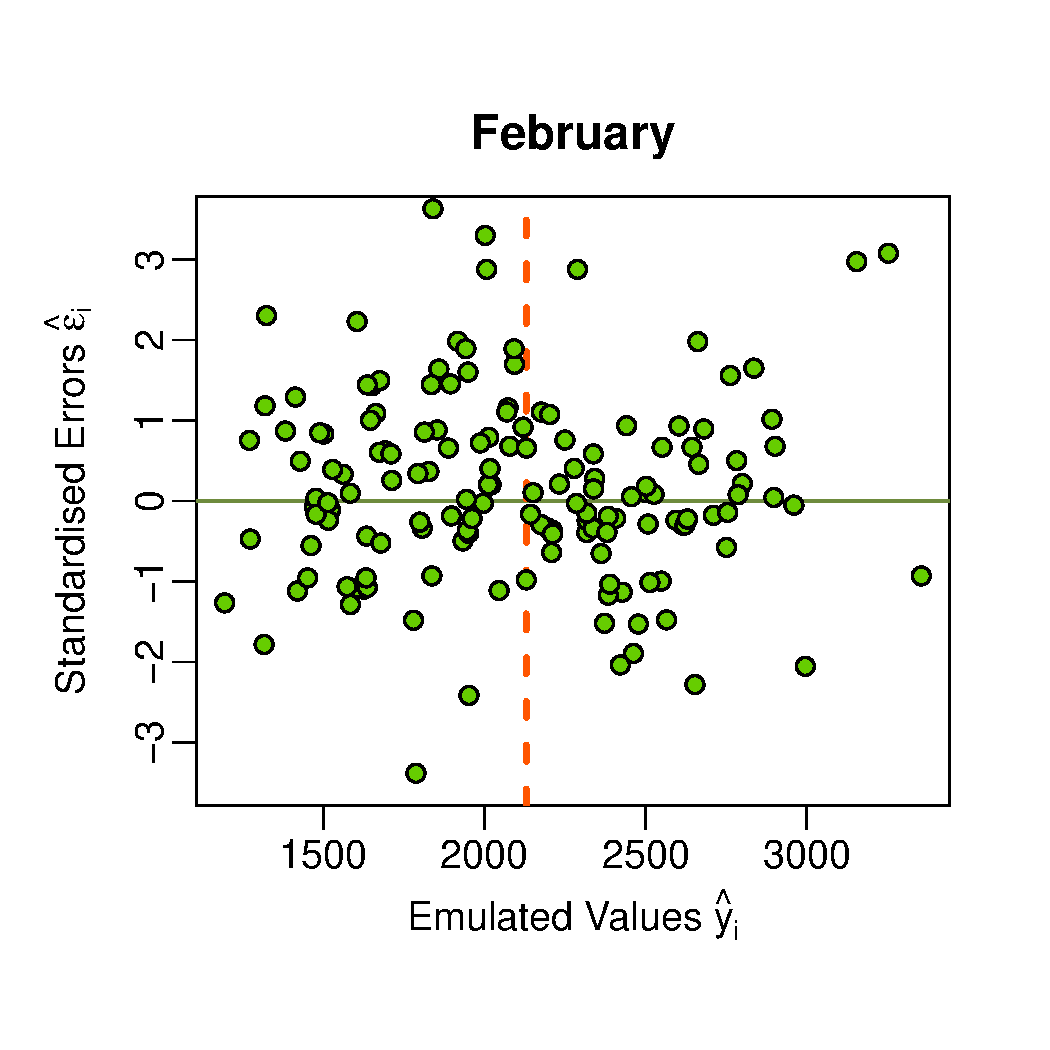
\includegraphics[width=\scale]{Validation_Plots/Evaluation_Set/Evaluation_Scatter_02_Feb}\hspace{-1ex}
 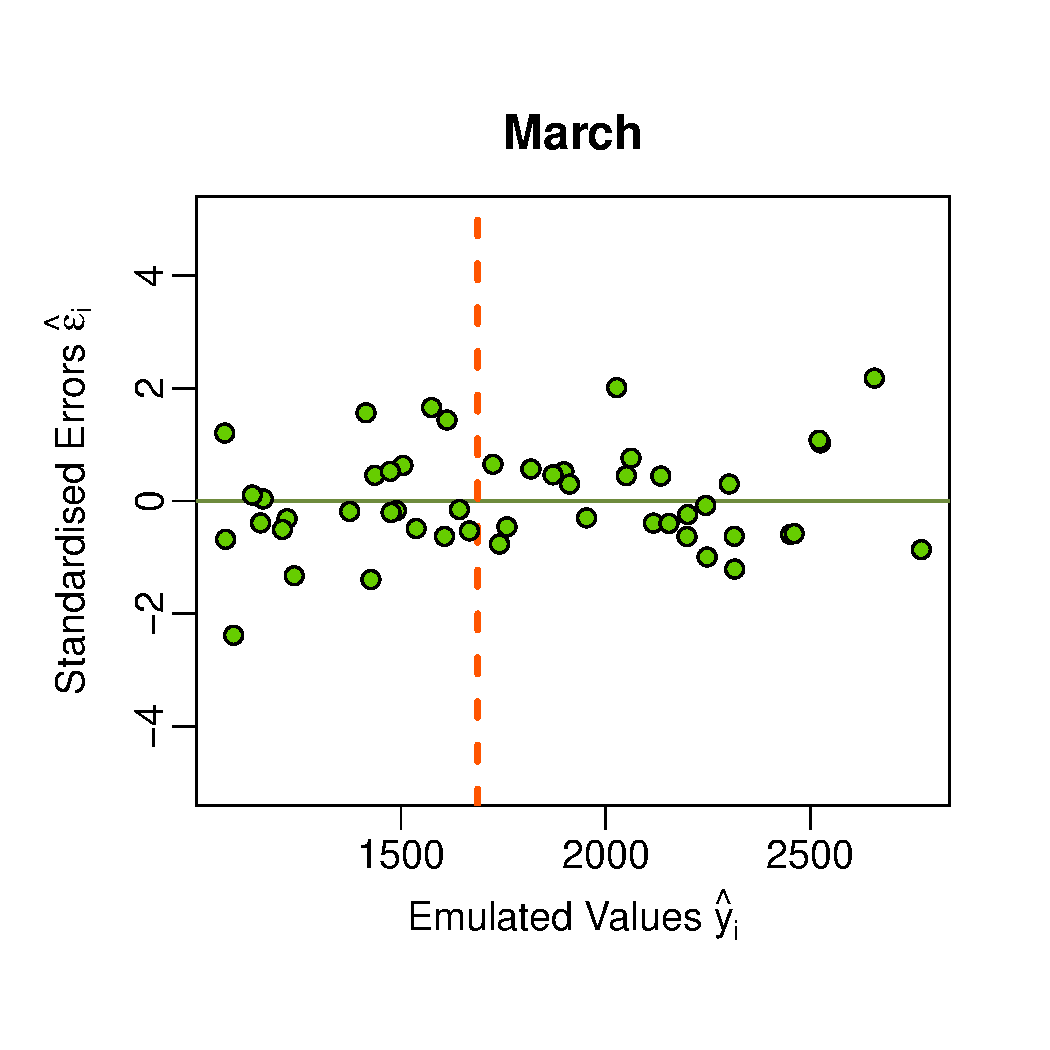
\includegraphics[width=\scale]{Validation_Plots/Evaluation_Set/Evaluation_Scatter_03_Mar}\\[-3ex]
 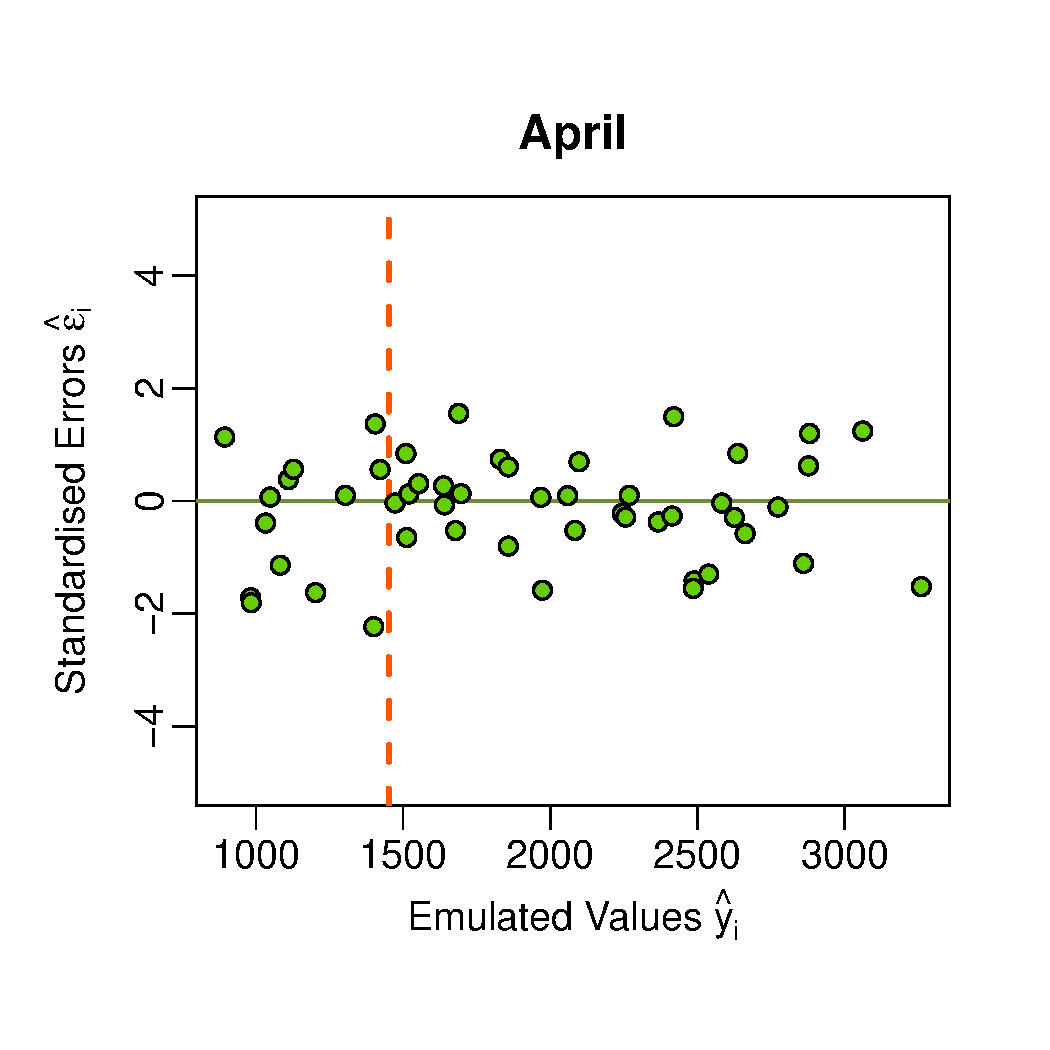
\includegraphics[width=\scale]{Validation_Plots/Evaluation_Set/Evaluation_Scatter_04_Apr}\hspace{-1ex}
 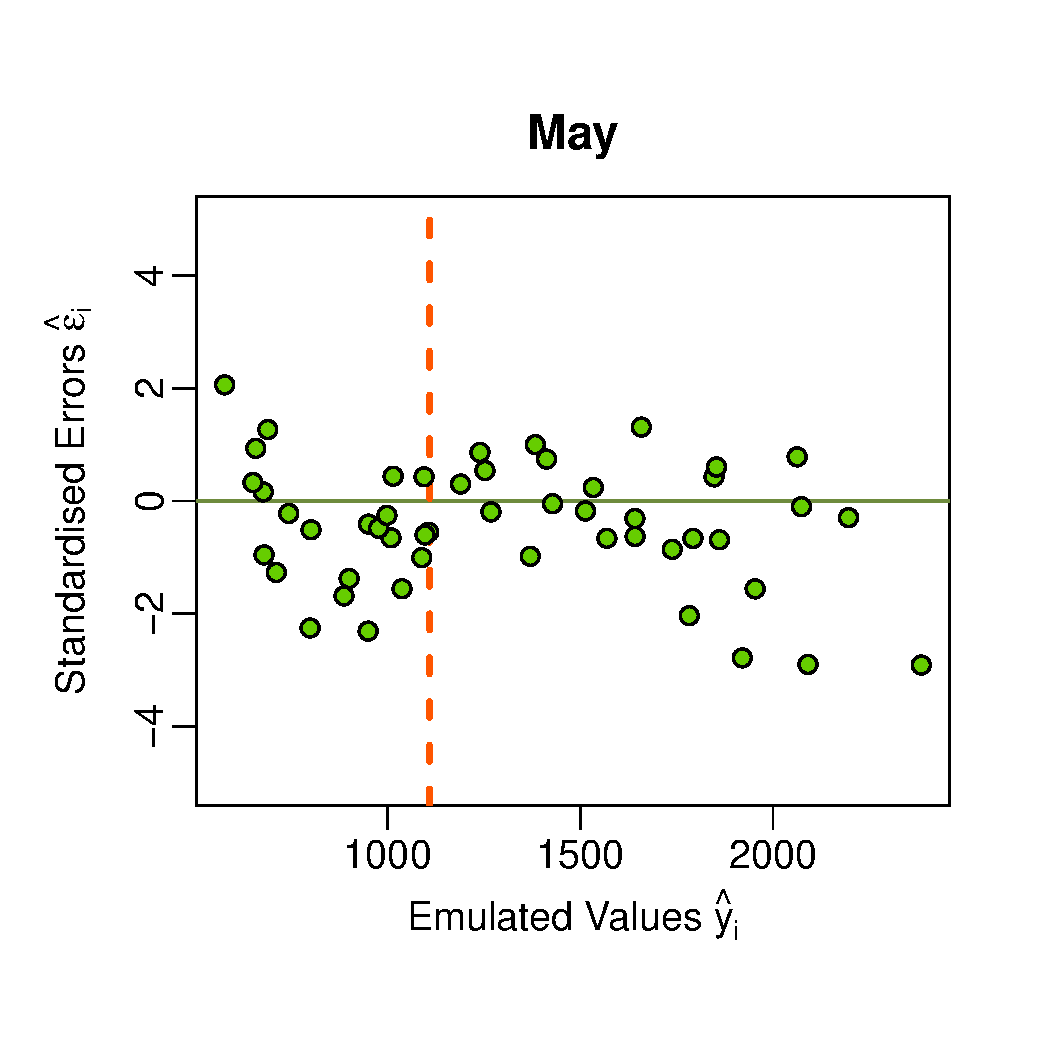
\includegraphics[width=\scale]{Validation_Plots/Evaluation_Set/Evaluation_Scatter_05_May}\hspace{-1ex}
 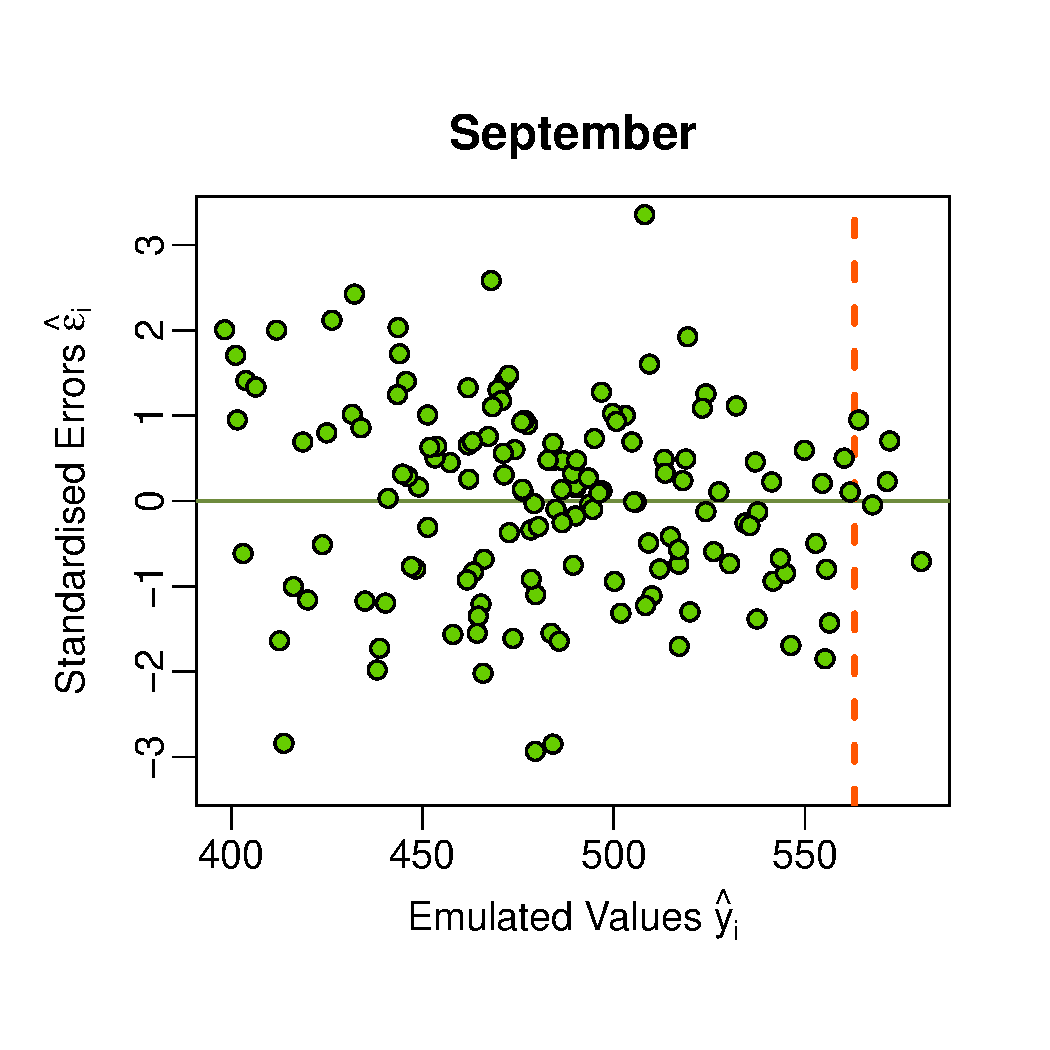
\includegraphics[width=\scale]{Validation_Plots/Evaluation_Set/Evaluation_Scatter_09_Sep}\\[-3ex]
 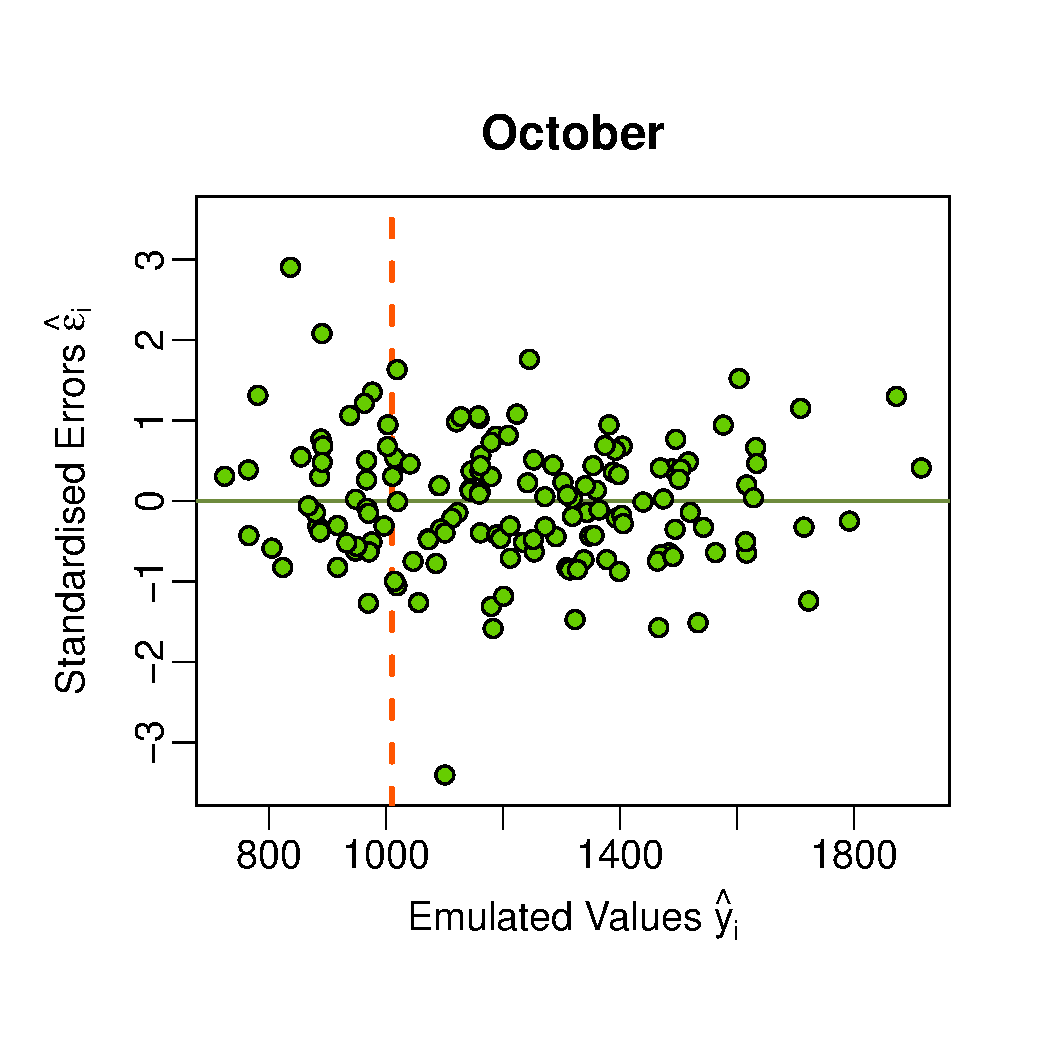
\includegraphics[width=\scale]{Validation_Plots/Evaluation_Set/Evaluation_Scatter_10_Oct}\hspace{-1ex}
 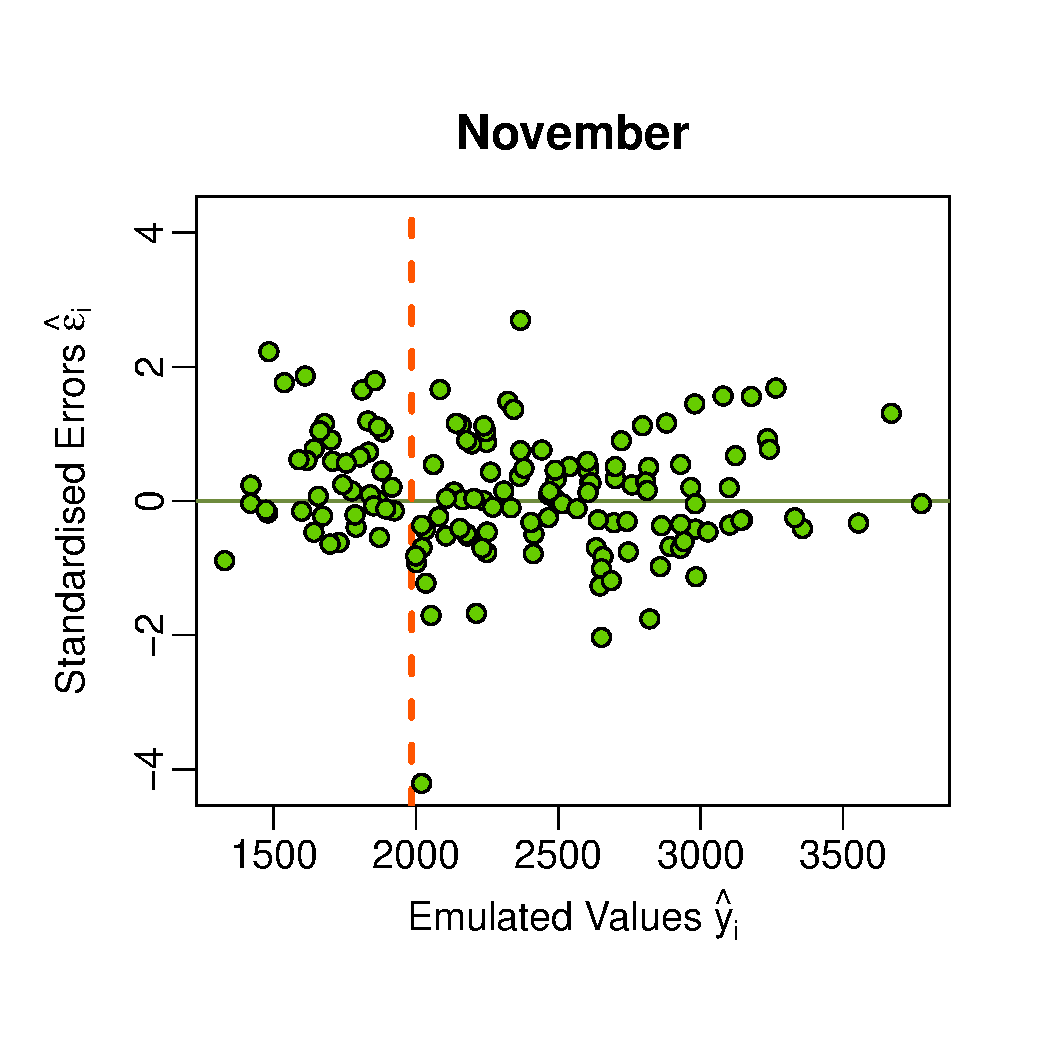
\includegraphics[width=\scale]{Validation_Plots/Evaluation_Set/Evaluation_Scatter_11_Nov}\hspace{-1ex}
 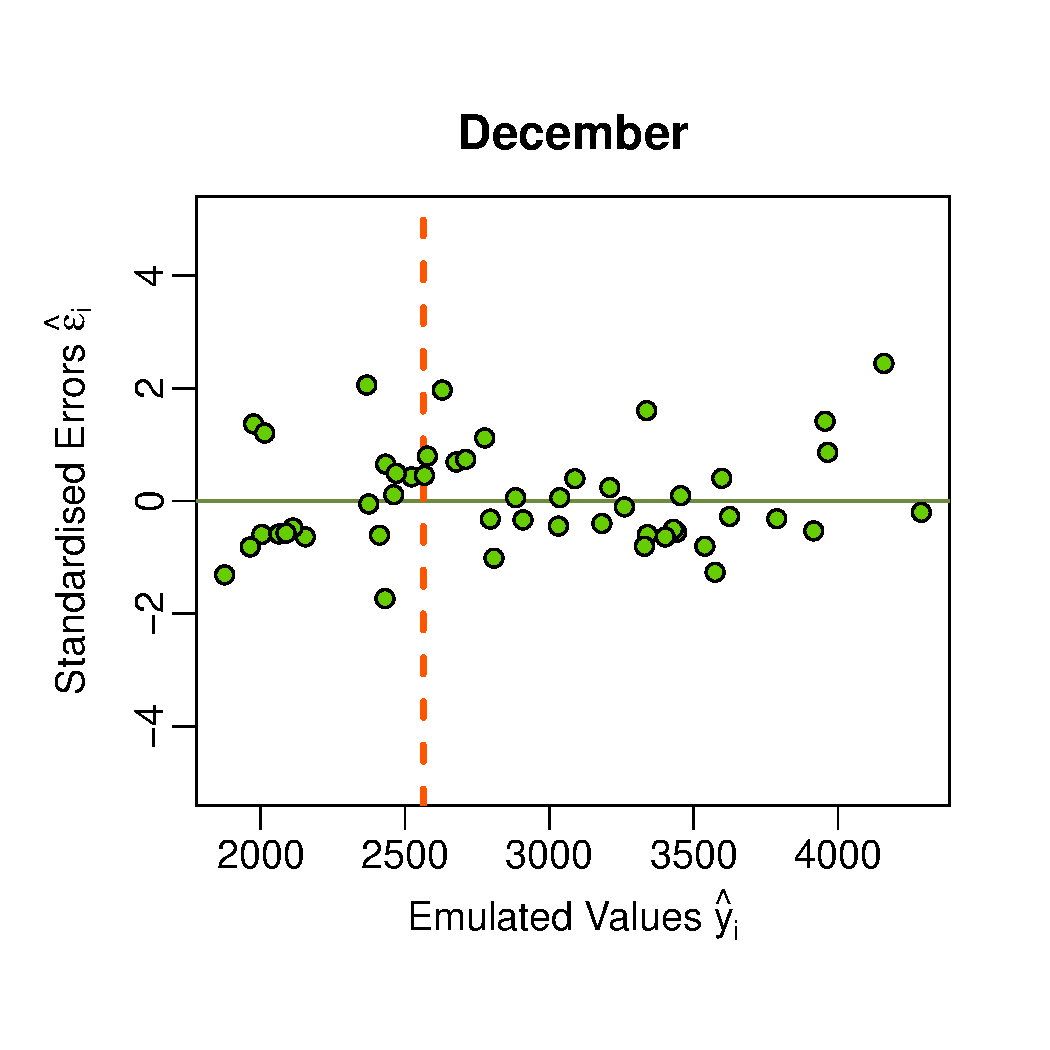
\includegraphics[width=\scale]{Validation_Plots/Evaluation_Set/Evaluation_Scatter_12_Dec}
 \caption{Validation of the emulators on the evaluation set, consisting of 150 points not used in training. For the different months, the standardised errors in \eqref{Eqn_St_Er} are plotted against the emulator's fitted values. In each plot, the vertical dashed line identifies the value on the $x$-axis corresponding to the observed gas consumption for the month.}
 \label{Fig_Scatter_Errors_Eval}
\end{figure}


\autoref{Fig_Scatter_Errors_Eval} and \autoref{Fig_Scatter_Errors_Test} show the emulated standardised errors on the evaluation and test sets respectively. For any point in such sets, call $y_i$ the known simulator response, $\hat{y}_i$ the emulator prediction and $\hat{\sigma}_i$ the associated standard deviation. The standardised error is computed as follows:
\begin{equation}\label{Eqn_St_Er}
\hat{\eps}_i = \frac{y_i - \hat{y}_i}{\hat \sigma_i}.
\end{equation}

Values of the emulator hyperparameters have been chosen so that the standardised errors in \autoref{Fig_Scatter_Errors_Eval} would display as unstructured as possible patterns, and at least 95\% of them would be lower than 3 in modulus. We consider the plots in \autoref{Fig_Scatter_Errors_Eval} satisfactory in this regard. Only the plot concerning May displays a few larger errors, particularly for low $\hat y$ values. This may be a sign that the simulator response varies non-linearly between parts of the space corresponding to smaller and bigger $y$ values. Moreover, further investigation shows that the point with lowest (negative) $\hat \eps$ in the seven plots January--April and October-December corresponds to the same choice of inputs in all cases. The point, then, may be considered an outlier with respect to the emulator models, although its standardised errors rarely go beyond the value $-4$. As to all other points, their standardised errors are essentially comprised between $-3$ and $+3$. 

The plots in \autoref{Fig_Scatter_Errors_Test} show the standardised errors of a set of completely new points, not used in training or evaluation. The plots show that the magnitude and pattern of the standardised errors are satisfactory for the test set too, so we consider the emulators successfully validated.


\begin{figure}
\centering
 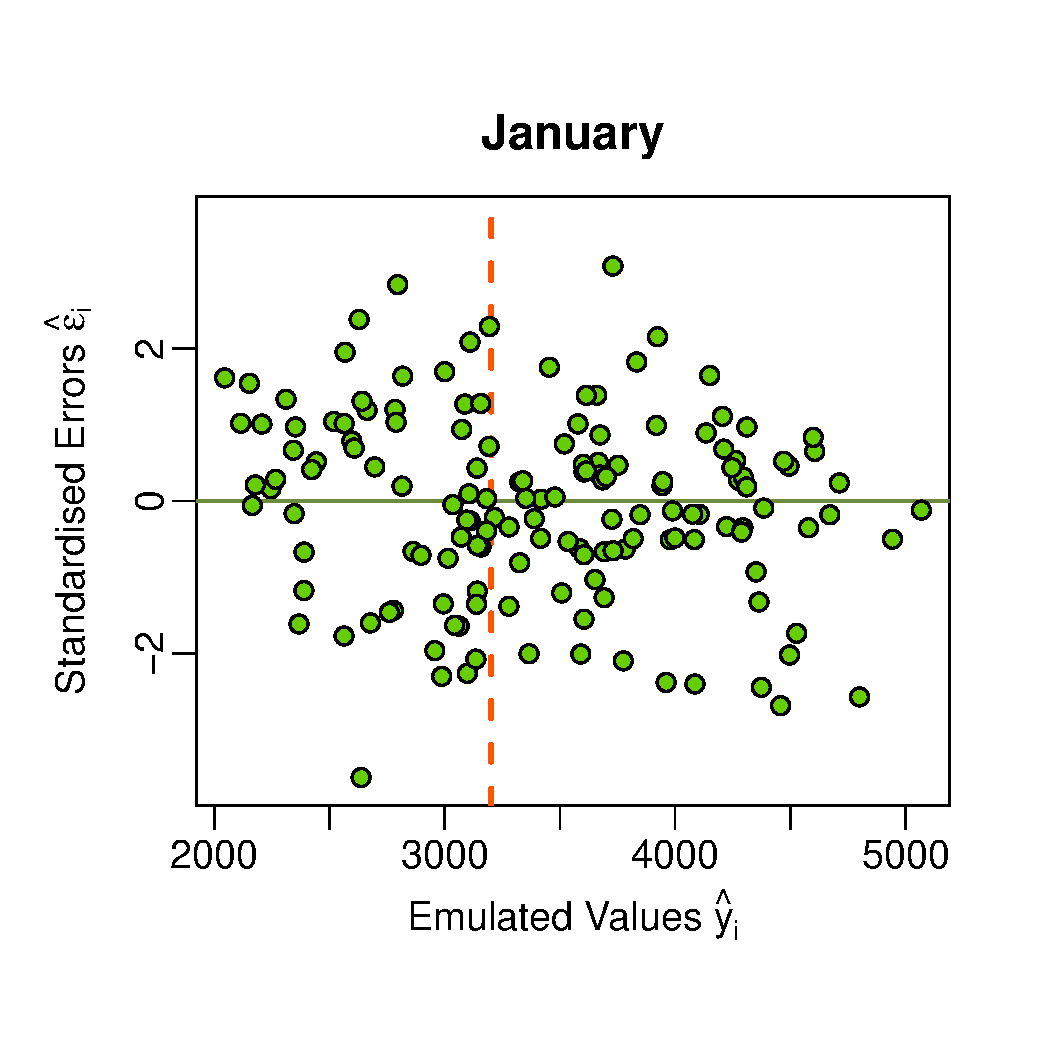
\includegraphics[width=\scale]{Validation_Plots/Test_Set/Test_Scatter_01_Jan}\hspace{-1ex}
 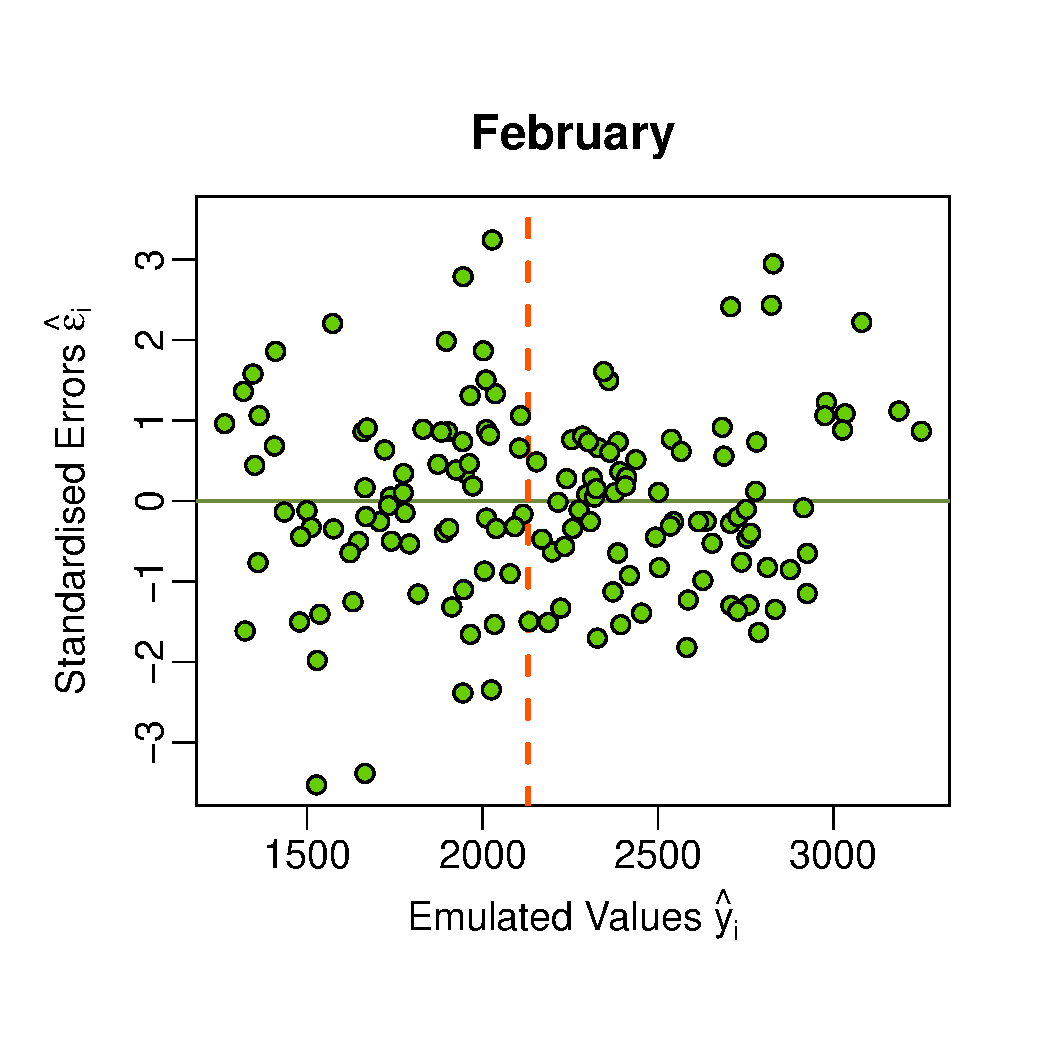
\includegraphics[width=\scale]{Validation_Plots/Test_Set/Test_Scatter_02_Feb}\hspace{-1ex}
 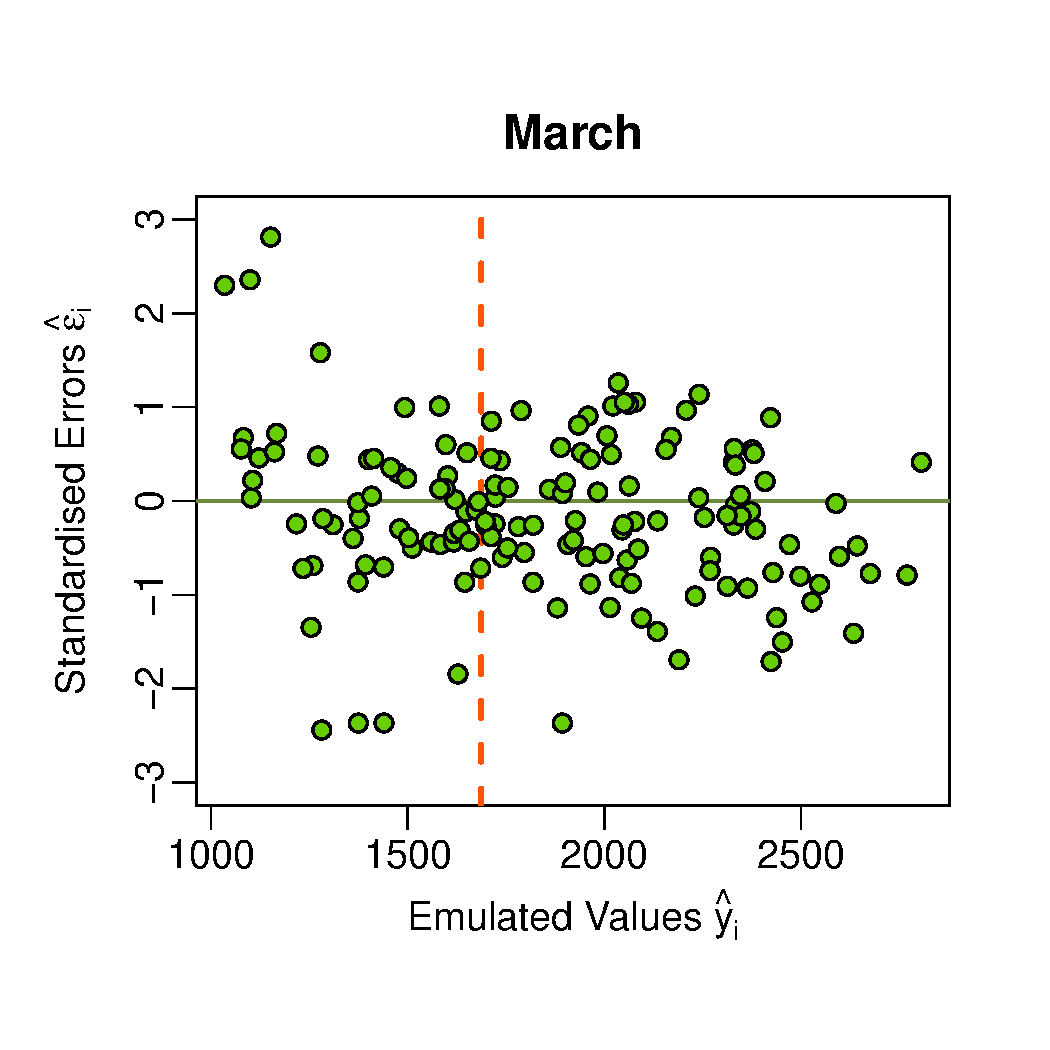
\includegraphics[width=\scale]{Validation_Plots/Test_Set/Test_Scatter_03_Mar}\\[-3ex]
 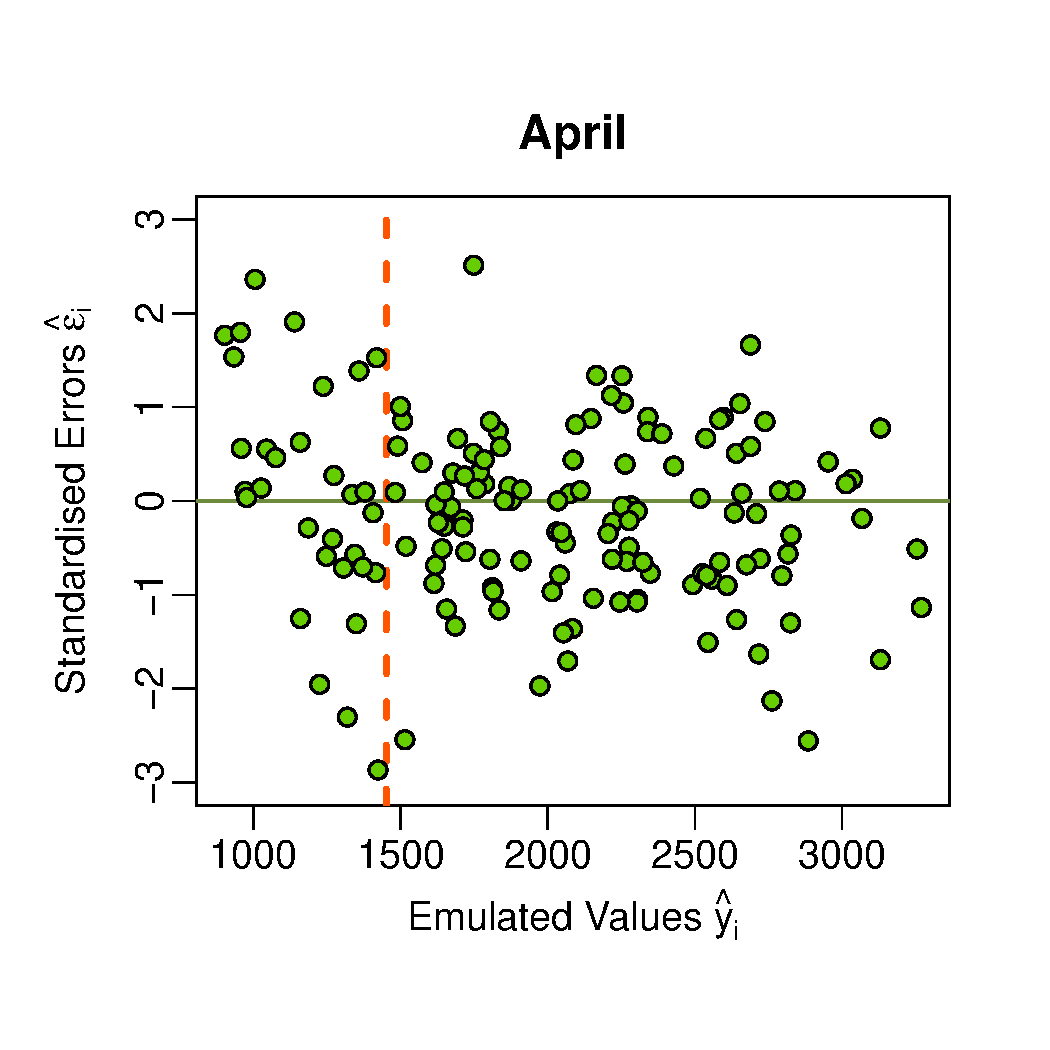
\includegraphics[width=\scale]{Validation_Plots/Test_Set/Test_Scatter_04_Apr}\hspace{-1ex}
 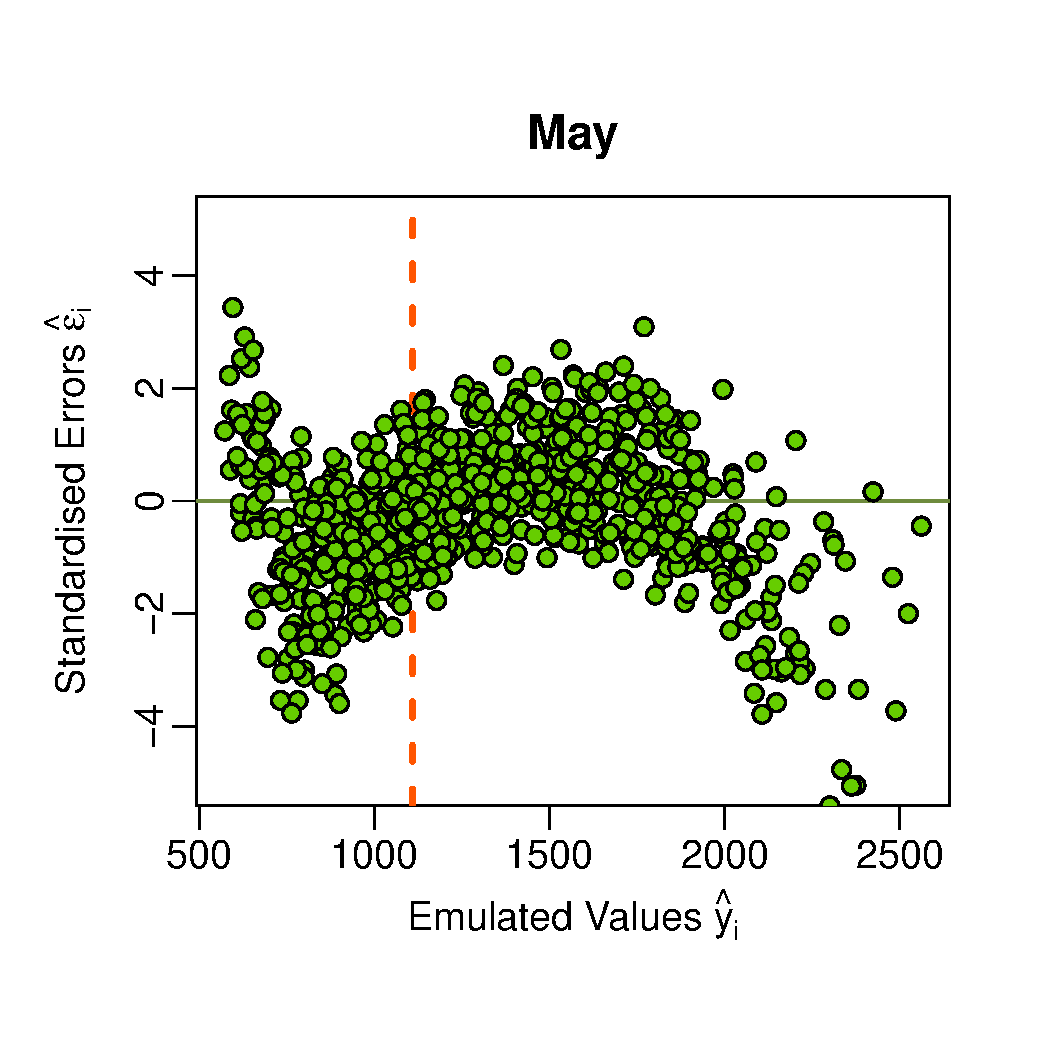
\includegraphics[width=\scale]{Validation_Plots/Test_Set/Test_Scatter_05_May}\hspace{-1ex}
 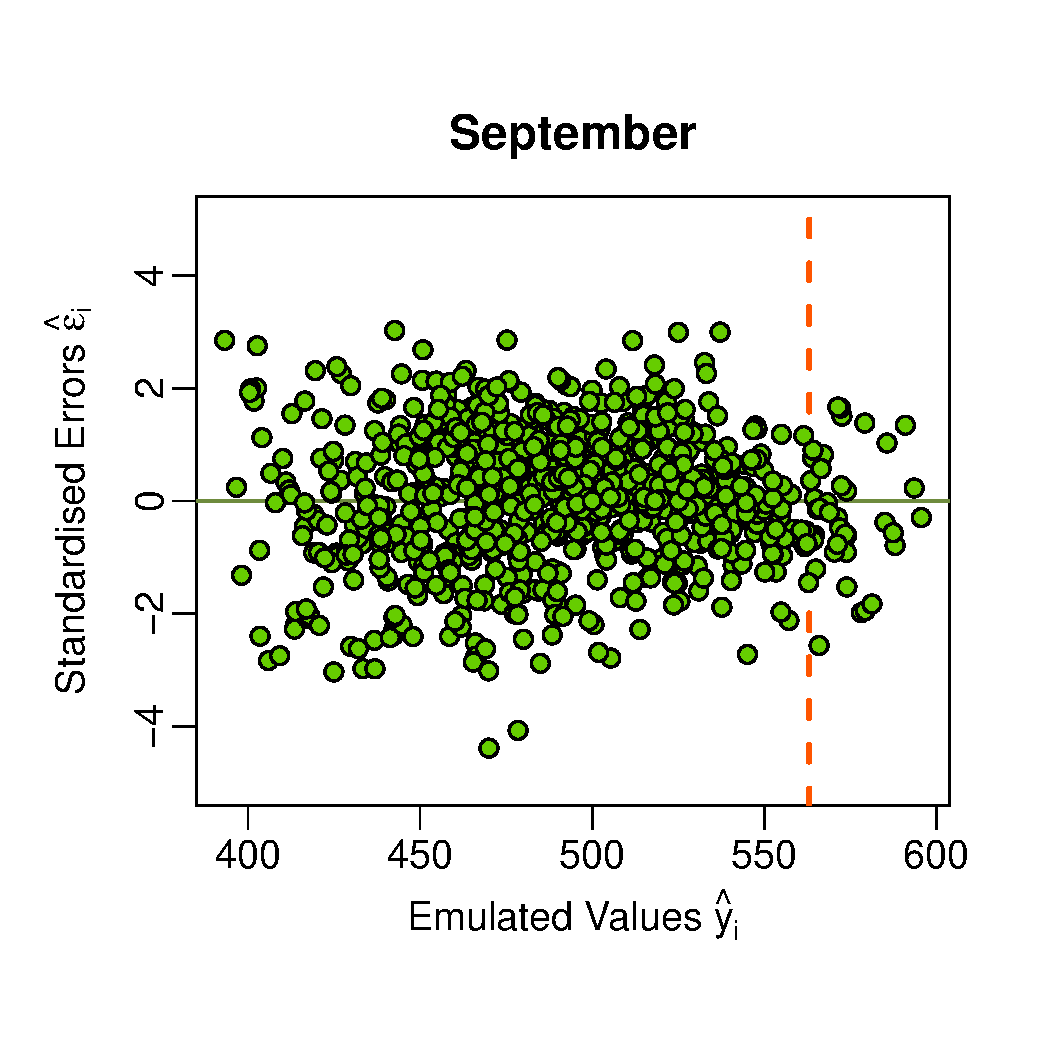
\includegraphics[width=\scale]{Validation_Plots/Test_Set/Test_Scatter_09_Sep}\\[-3ex]
 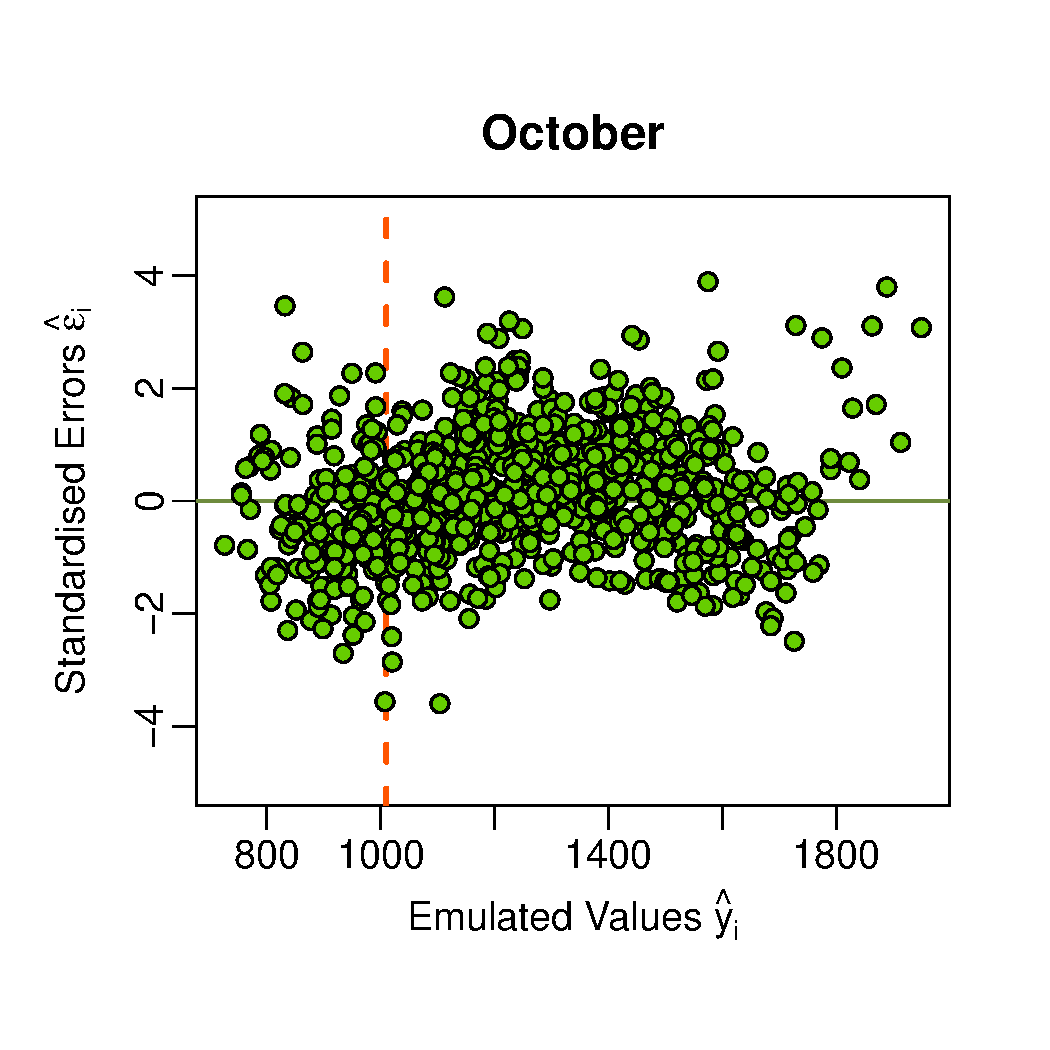
\includegraphics[width=\scale]{Validation_Plots/Test_Set/Test_Scatter_10_Oct}\hspace{-1ex}
 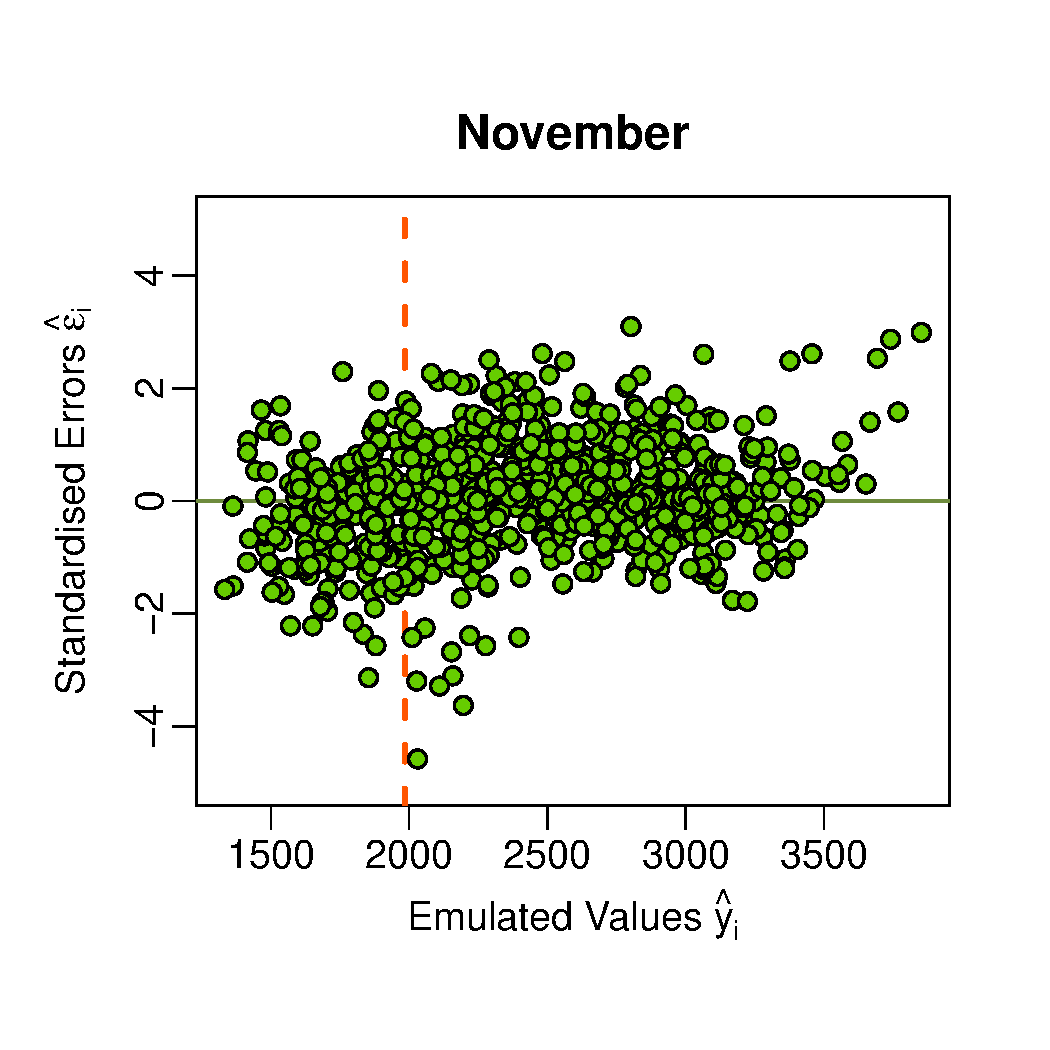
\includegraphics[width=\scale]{Validation_Plots/Test_Set/Test_Scatter_11_Nov}\hspace{-1ex}
 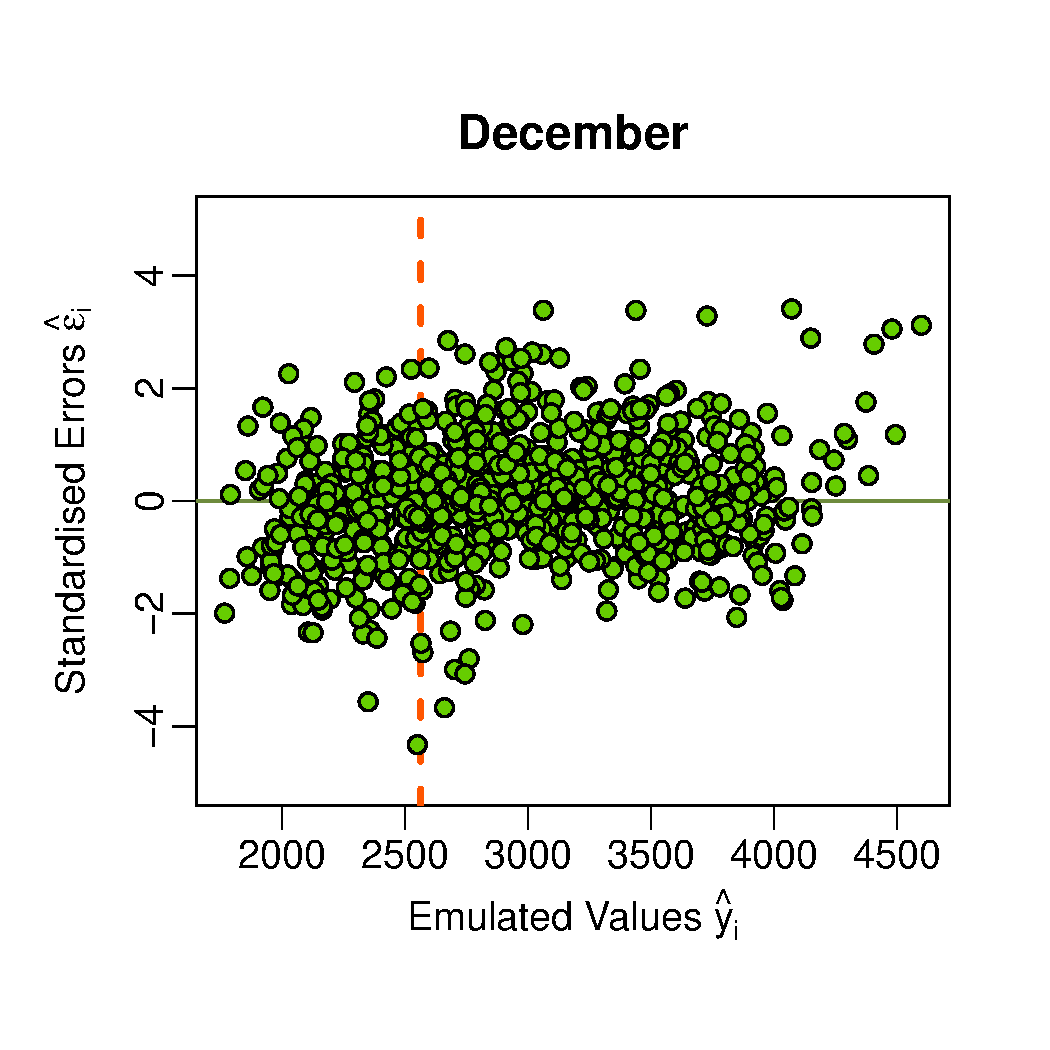
\includegraphics[width=\scale]{Validation_Plots/Test_Set/Test_Scatter_12_Dec}
\caption{Validation of the emulators on the test set, consisting of 150 points not used in training and evaluation. For the different months, the standardised errors in \eqref{Eqn_St_Er} are plotted against the emulator's fitted values. In each plot, the vertical dashed line identifies the value on the $x$-axis corresponding to the observed gas consumption for the month.}
 \label{Fig_Scatter_Errors_Test}
\end{figure}


\subsection{Comparison Between LR and Trained Emulators}

For each month, \autoref{Table_sigma} compares the prior variance of the emulator (\ie, the variance of the original linear regression residuals) with the adjusted variance of the emulator predictions on the 150 test points. I am reporting the $2.5$ and $97.5$ empirical percentiles of these, to get a sense of the difference in prediction uncertainty between the original linear regression and the trained emulators.

\begin{table}
 \centering
 \renewcommand{\arraystretch}{1.7}
 \newcommand{\colsep}{3ex}
 \tabcolsep=6pt
 \caption{For each month: the first line of the table shows the variance of the linear regression residuals (prior cumulative variance of the emulator). The second and third lines show the $2.5$ and $97.5$ empirical percentiles of the emulator variances at the 150 test points.}
 \begin{tabular}{c<{\hspace{\colsep}}ccccccccc}
\specialrule{.1em}{0em}{0.1em} 
 &  \textbf{Jan} & \textbf{Feb} & \textbf{Mar} & \textbf{Apr} & \textbf{May} & \textbf{Sep} & \textbf{Oct} & \textbf{Nov} & \textbf{Dec}\\
 \specialrule{.05em}{.1em}{0.1em} 
 \specialrule{.05em}{0em}{0.2em} 
  $\sigma^2$  & 85.9 &  52.3  &  50.1 &  50.0  & 206.4  &  0.91 &  24.4  & 57.4  &  68.8\\
  $[2.5\%$,       & 6.6   & 5.9     &  3.1   & 3.2      & 16.8    & 0.06  & 1.46   & 3.8    & 4.3\\
  $97.5\%]$ CI & 31.0 & 28.0   & 9.3    & 10.0   & 68.9    &  0.20 & 3.80   & 12.8  & 12.7\\
 \specialrule{.1em}{0.2em}{1em} 
 \end{tabular}
\label{Table_sigma}
\end{table}

Finally, \autoref{Fig_Comparison_LR} allows to compare graphically the accuracy of the emulator's predictions versus the linear regression's ones. The plot concerns the month of March. Results for only 8 of the 150 test points are shown (8 consecutive ones in terms of the simulator outputs), to avoid cluttering which would prevent details to be appreciated. 

The red ``cat's eye'' boxes represent the emulator predictions for these points, within a range of three standard deviations from the mean prediction. The blue plus sign and the yellow squares represent instead the real simulator outputs and the linear regression predictions, respectively. It can be appreciated that the emulator is often much more precise than the linear model, and has a high level of confidence in its prediction (small uncertainty bands).




\begin{figure}
\centering
 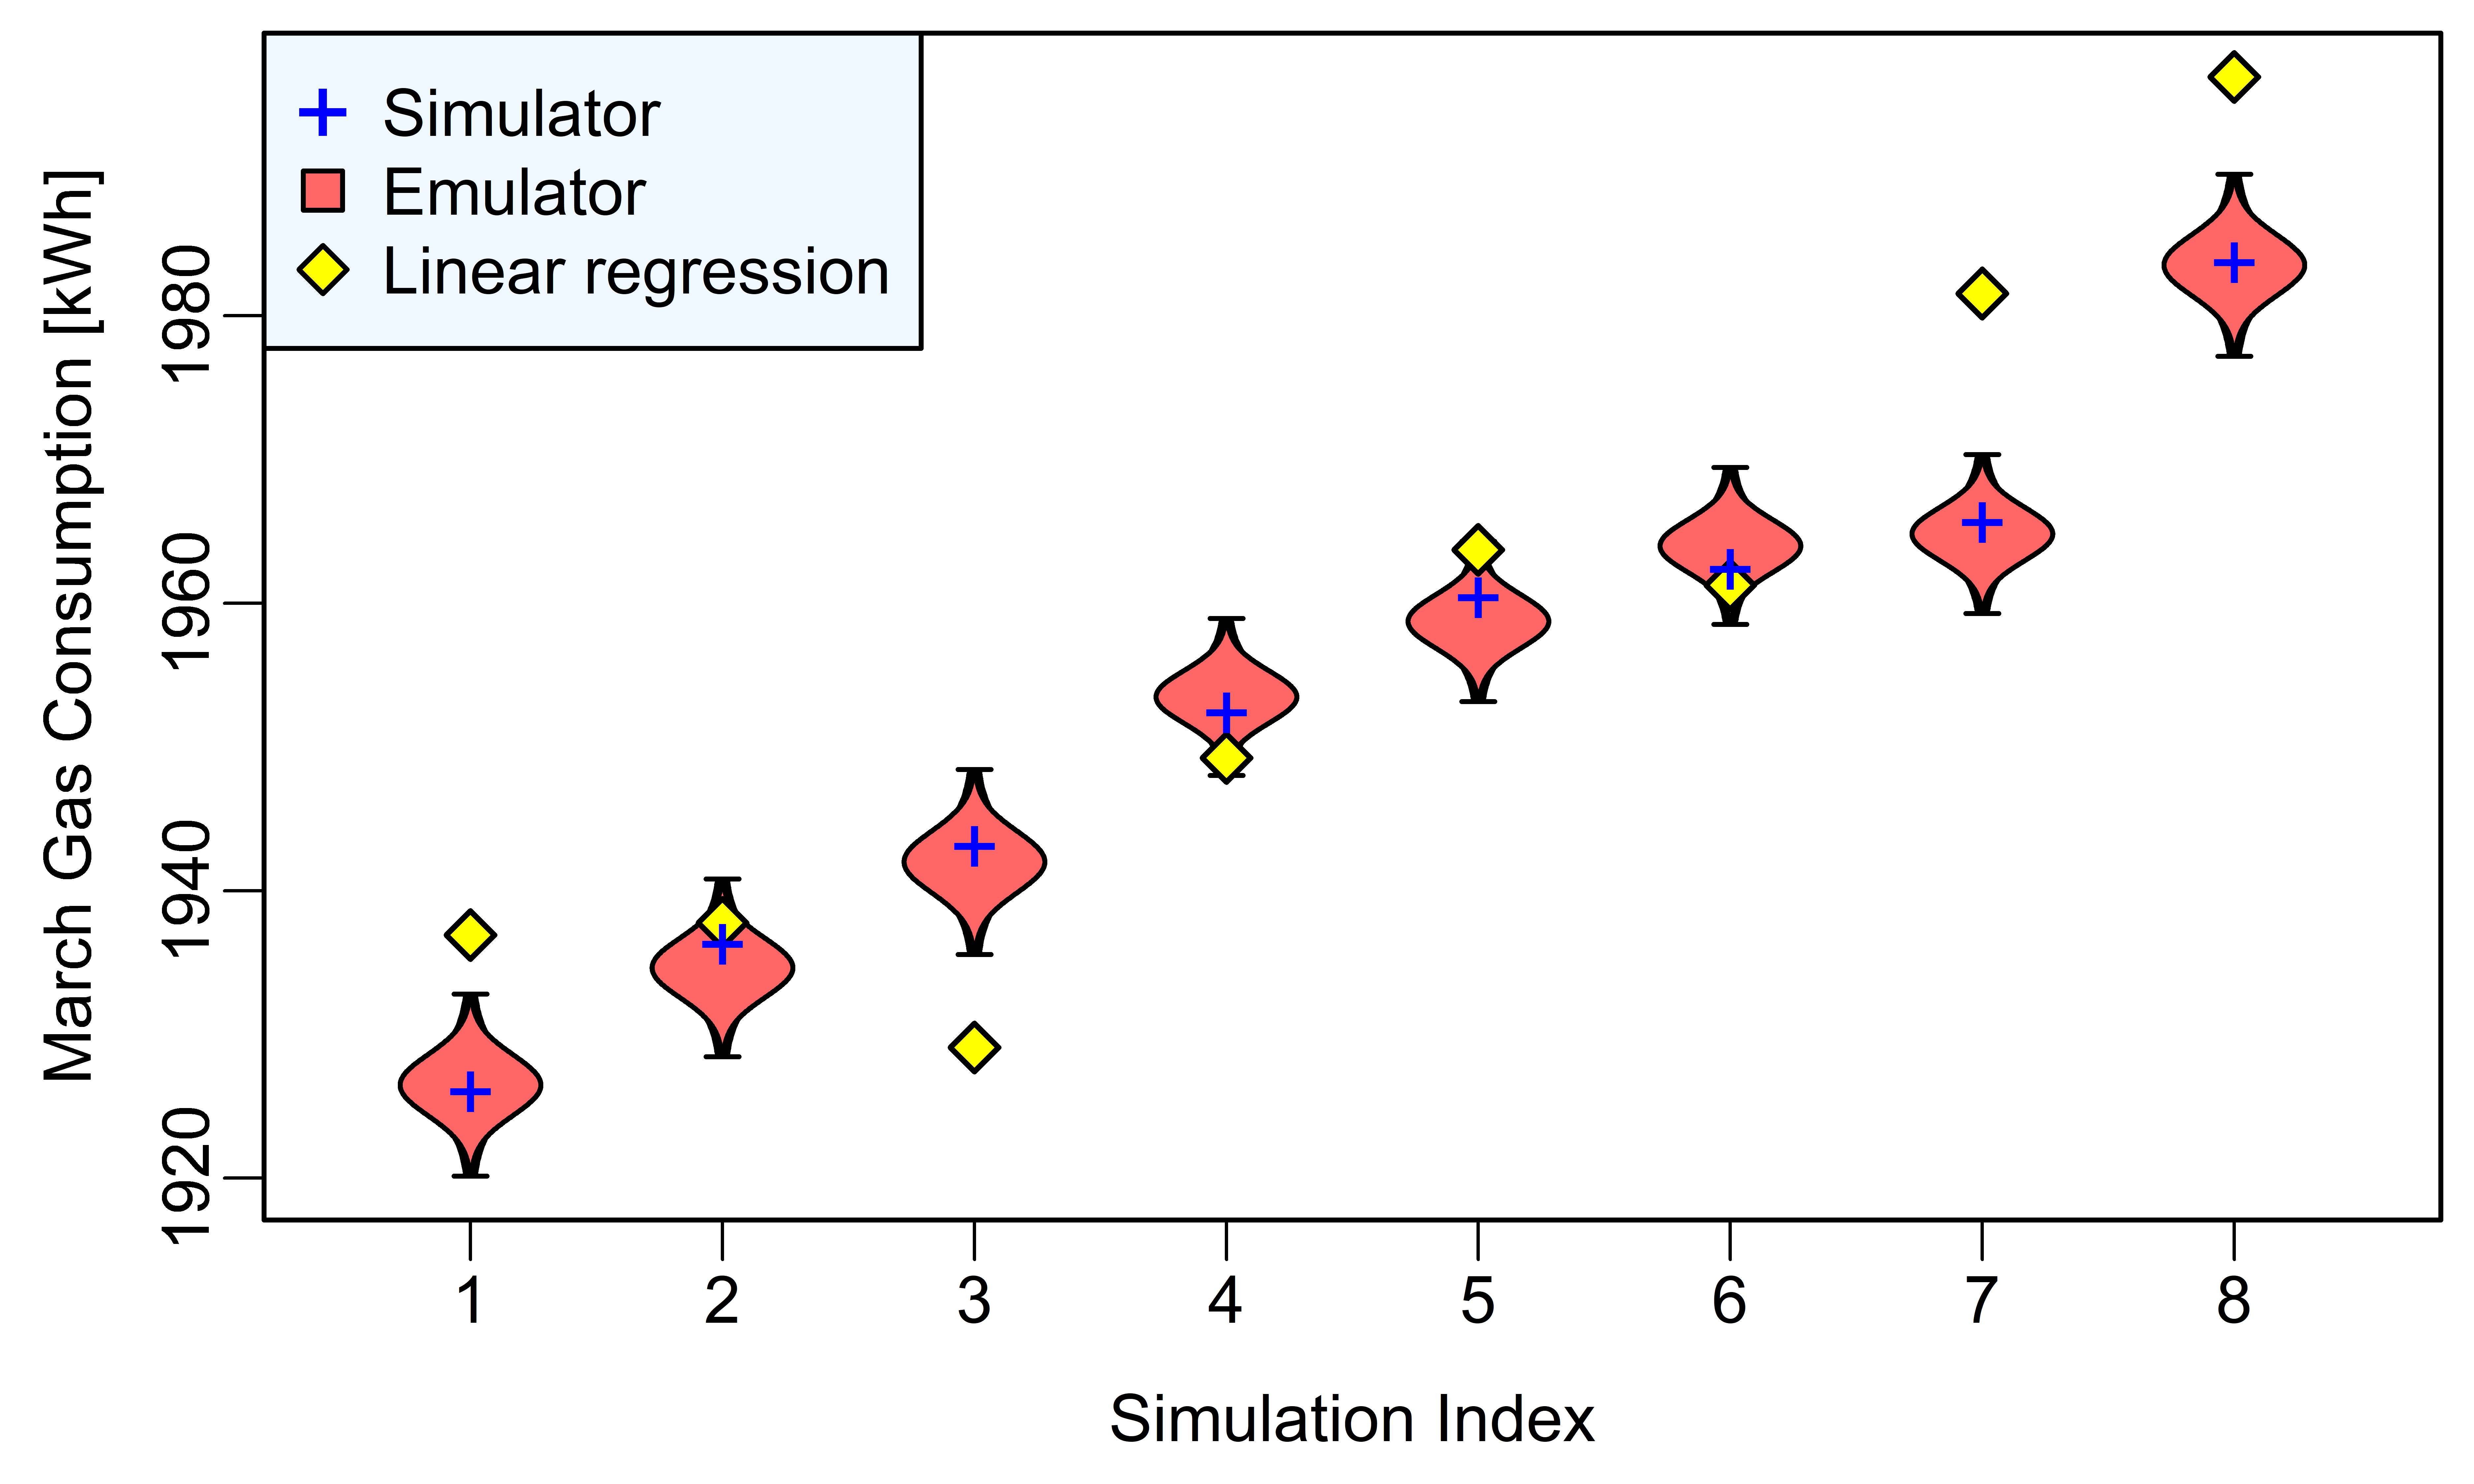
\includegraphics[width=0.8\textwidth]{Validation_Plots/Comparison_LR/LR_Mar_82-89}
 \caption{Visual comparison between emulator (red cat's eye boxes) and linear regression (yellow squares) predictions. The plot concerns 8 points of the test set for the month of March. The height of the emulator cat's eye boxes covers a range of three standard deviations from the emulator's mean prediction. This range always includes the simulated value (blue plus sign), and often represents a much more precise prediction than the original linear regression one.}
 \label{Fig_Comparison_LR}
\end{figure}




\section{History Matching}

The emulators built and validated in previous sections allow to predict, for any input $\x \in \R^8$, the simulated gas consumption $f(\x)$ associated with that set of inputs.
Since observed gas consumptions are available for each month, we can use the emulators to select inputs $\x$ whose simulated gas consumptions are ``compatible'' with the observed data.
The context and notation to carry out the comparison are introduced below. 


\subsection{Notation and Choices}
Let $f(\x)$ denote the simulated gas consumption associated with input $\x$. With a slight abuse of notation which should however cause no confusion, we denote by $\E[f(\x)]$ and $\Var[f(\x)]$ the emulator mean prediction and variance associated with input $\x$. Finally, we denote by $z \in \R$ the observed gas consumption. Note that, albeit not explicitly signalled in the notation, all these quantities depend on the particular month considered.


When using the emulator to assess the compatibility between the (unknown) value $f(\x)$ corresponding to a given input $\x$, and the available observed consumption $z$, we need to account for at least three different types of uncertainties.
\begin{enumerate}
 \item The emulator prediction is only an approximation to the actual model response
       $f(\x)$: this uncertainty is naturally quantified by the emulator standard deviation associated with the prediction.
 \item Even if the emulator were a perfect reproduction of the simulator, the latter
       would only be an imperfect reproduction of reality. We ultimately want to learn about the real world, so model discrepancy (MD) should be accounted for.
 \item Due to unavoidable measurement errors (MEs), the observed consumption $z$
       differs from the actual amount of gas consumed in the building during the month.
\end{enumerate}

The aim of the first wave of emulators is to discard those inputs $\x$ which, once the previous uncertainties are accounted for, are extremely unlikely to lead to gas consumption $z$ in the real world. In order to quantify the mismatch between an input $\x \in \R^8$ and the observed $z$ for the month $M$, we consider the following implausibility measure\footnote{
I don't add much here, but clearly in a paper we would reference Michael's work and possibly restructure the exposition.}:
\begin{equation}
 I_M(\x) = \frac{\big|\, \E[f(\x)] - z \,\big| }{ \sqrt{
 {\Var[f(\x)]}^{\phantom{i}} \!+ \Var[\epsilon_{_\text{MD}}(\x)] + \Var[\epsilon_{_\text{ME}}(z)] \,}^{\,}
       } \,, \;\quad \x \in \R^8.
\end{equation}
The subscript $M$ denotes the dependence on the month considered (it is omitted from the terms on the right-hand side for simplicity of notation).
The quantity $I_M(\x)$ is dimensionless. The last two terms of the denominator represent the uncertainty ascribed to model discrepancy and measurement errors respectively, and have the same dimension as $\Var[f(\x)]$.


In our case, we assess the measurement error to be of the order of $5\%$ of the reported gas consumption $z$. To translate this into a value for $\Var[\epsilon_{_\text{ME}}]$, we
make the simplifying assumption that the actual consumption has uniform probability of being anywhere in the interval $[0.975 z, 1.025 z]$. Since the variance of a uniform random variable on an interval of length $L$ is $L^2/12$, this assumption yields:
\begin{equation}
 \Var[\epsilon_{_\text{ME}}(z)] = \frac{z^2}{\,4800\,}\,.
\end{equation}

As far as model discrepancy is concerned, we consider three different scenarios, where the discrepancy between a simulated output $y$ and reality is estimated in about $5\%$, $10\%$ and $20\%$ of $y$ respectively. Since the output $y$ is not available for a general input $\x$, we consider the quantity $\E[f(\x)]$ as its surrogate, therefore computing $\Var[\epsilon_{_\text{MD}}(\x)]$
as
\begin{equation}
\frac{ \,{\E[f(\x)]}^2\, }{4800}\,, \;
\frac{ \,{\E[f(\x)]}^2\, }{1200}\,, \;
\frac{ \,{\E[f(\x)]}^2\, }{300}
\end{equation}
in the three scenarios respectively.



For the month $M$, we define an input $\x$ as ``non-implausible for $M$'' if the value $I_M(\x)$ is lower than a given threshold $T$. Hence, it is natural to define an input as ``non-implausible'' if the previous condition holds true for all the months. That is, if
\begin{equation}\label{Condition}
\max_{M \in \mathcal{M}} \big\{ I_M(\x) \big\} < T\,,
\end{equation}
where $\mathcal{M}$ is the set of nine months considered in this work. Since the previous equation represents the simultaneous imposition of nine conditions, we consider two fairly conservative values of $T$ in equation~\eqref{Condition}: $T=4$ and $T=5$.


\subsection{Results}

\begin{table}
 \centering
 \renewcommand{\arraystretch}{1.6}
 \setlength{\tabcolsep}{0.9ex}
 \caption{Percentages of non-implausible space when accounting for different size 
          of model discrepancy (MD). Results shown for two different values of the threshold $T$. In the ``All'' column, condition~\eqref{Condition} is used to classify a point as non-implausible.
          The looser condition $I_\text{M}(\x)<T$ is instead used in each of the remaining nine columns, for the different months ``M''
          (percentages rounded to the nearest integer). The ``$\approx 0$'' value in the table corresponds to $2.23 \times 10^{-6} \,\%$ of the space.
          }
 \begin{tabular}{c<{\hspace{2ex}} r<{\hspace{2ex}} ccccccccc}
 \specialrule{0.1em}{0em}{0.1em}
      & {\bf All} & {\bf Jan} & {\bf Feb} & {\bf Mar} & {\bf Apr} & {\bf May} & {\bf Sep} & {\bf Oct} & {\bf Nov} & {\bf Dec} \\
 \specialrule{0.05em}{0.1em}{0.1em}
 \specialrule{0.05em}{0em}{0.5em}
 \multirow{3}{*}{$T=4 \;\left\{ \begin{array}{r}
                                  5\% \text{ MD} \\
                                 10\% \text{ MD} \\
                                 20\% \text{ MD} 
                                \end{array}\right. $}    
                             & 0$\;\;$ & 24 & 24 & 21 & 13 & 14 & 26 & 20 & 19 & 22 \\
                             &   0.30  & 38 & 38 & 33 & 21 & 22 & 45 & 31 & 30 & 36 \\
                             & 19.52   & 70 & 69 & 63 & 39 & 42 & 81 & 59 & 57 & 67 \\
 \specialrule{0.05em}{0.5em}{0.5em}
 \multirow{3}{*}{$T=5 \;\left\{ \begin{array}{r}
                                  5\% \text{ MD} \\
                                 10\% \text{ MD} \\
                                 20\% \text{ MD} 
                                \end{array}\right. $}    
                         & $\approx 0$ & 30 & 30 & 26 & 16 & 18 & 35 & 25 & 24 & 28 \\
                         &    3.31     & 47 & 48 & 42 & 26 & 28 & 58 & 39 & 38 & 45 \\
                         &   37.02     & 84 & 81 & 78 & 50 & 54 & 92 & 74 & 72 & 82 \\ 
  \specialrule{0.1em}{0.5em}{0em}
\end{tabular}
 \label{Table_Implausibility}
\end{table}


\renewcommand{\scale}{18.8em}
\begin{figure}
\centering
 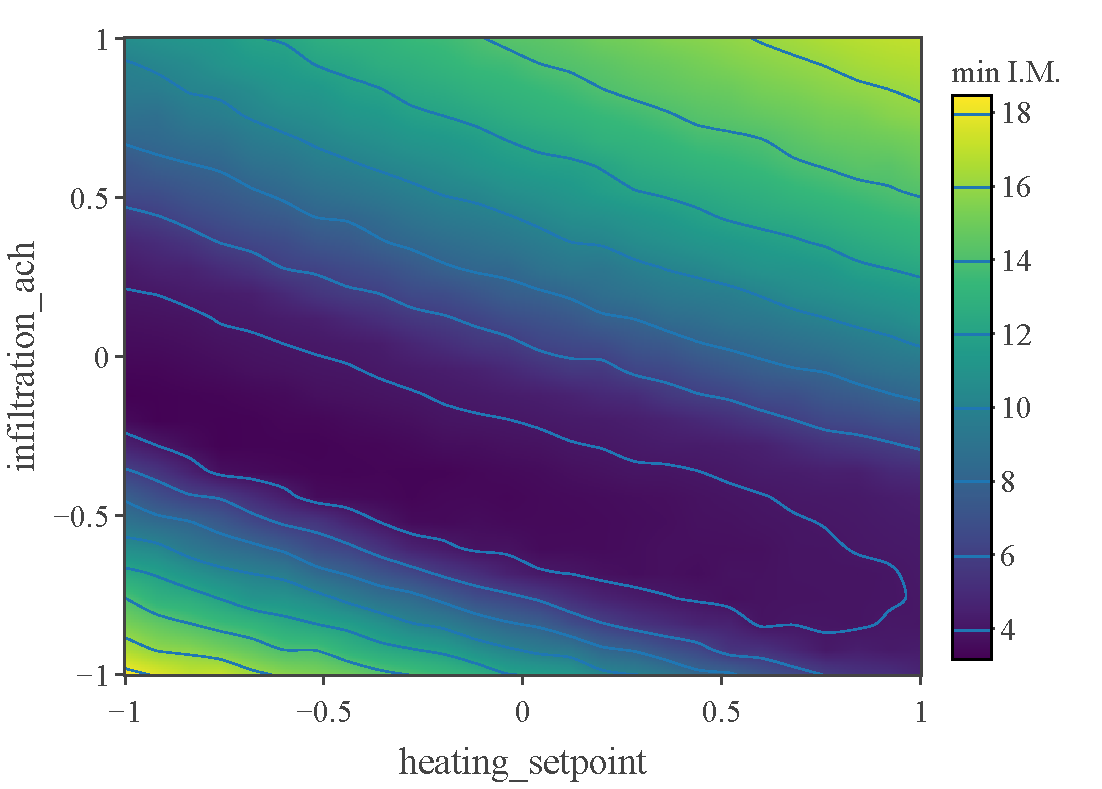
\includegraphics[width=\scale]{Gas_Compatibility/Min_Impl/minImpl_MD=10_x=1_y=6}
 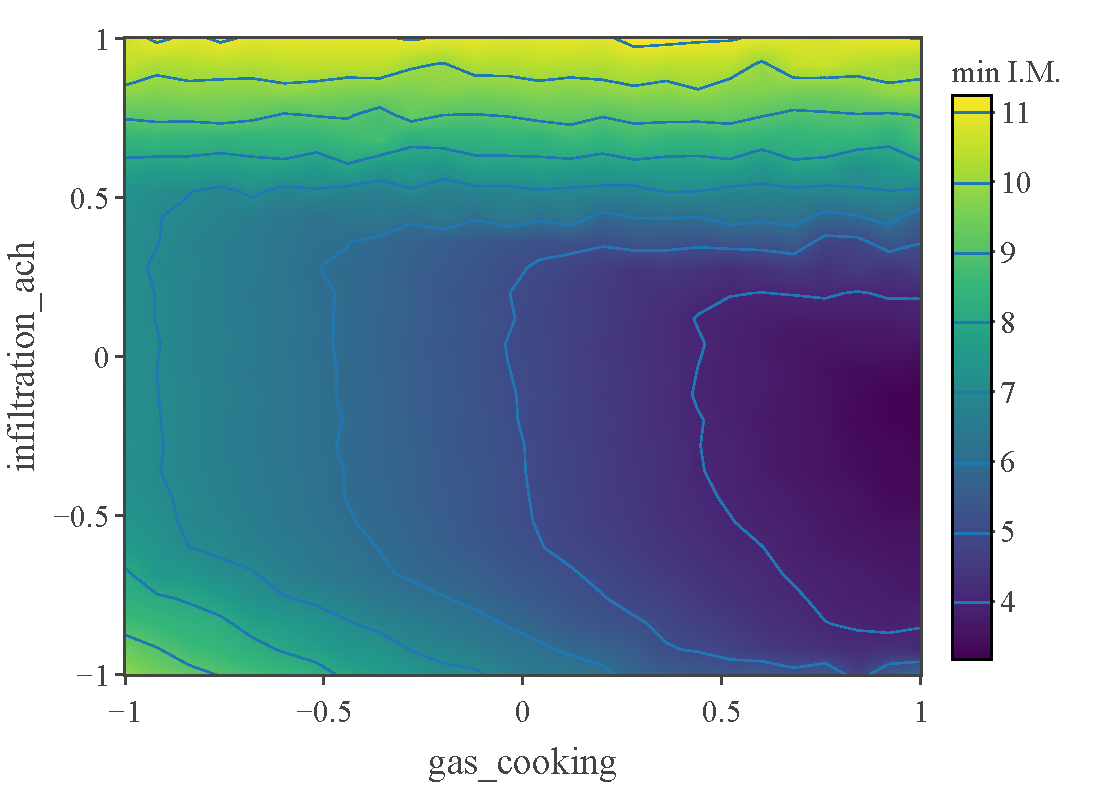
\includegraphics[width=\scale]{Gas_Compatibility/Min_Impl/minImpl_MD=10_x=8_y=6}\\
 \hspace{\scale}
  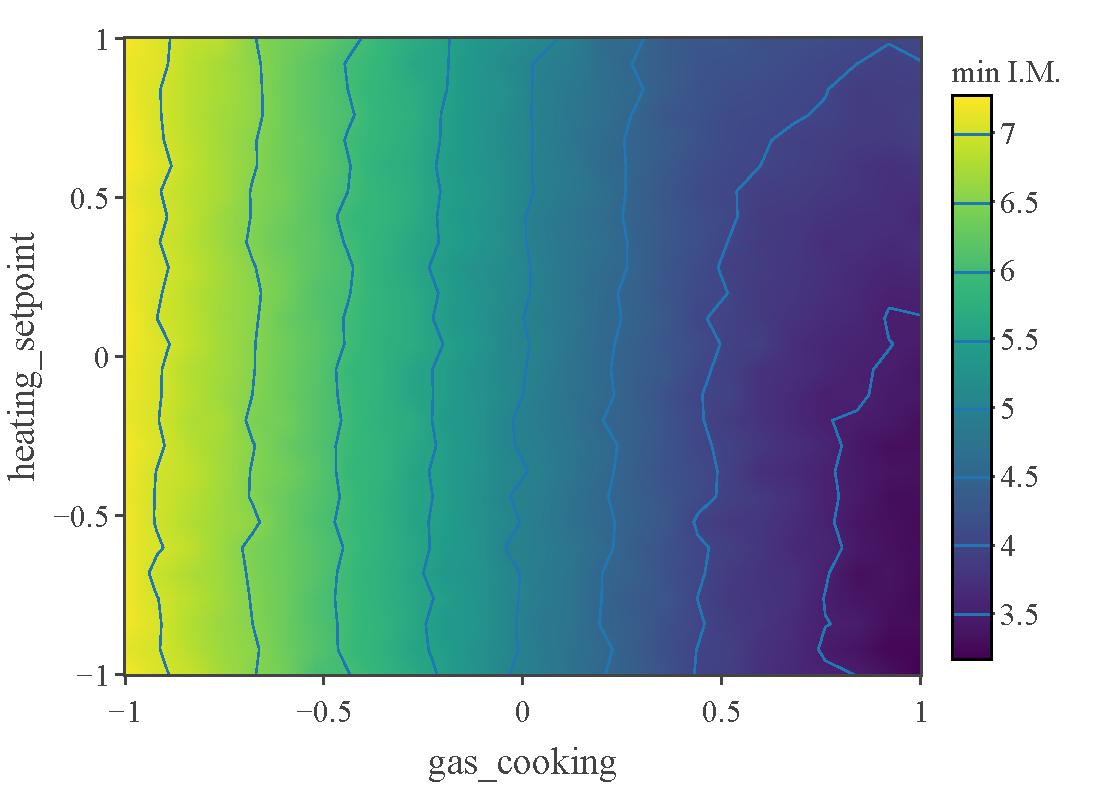
\includegraphics[width=\scale]{Gas_Compatibility/Min_Impl/minImpl_MD=10_x=8_y=1}
 \caption{10\% Model discrepancy}
 \label{Fig_Min_Implaus_10MD}
\end{figure}

\begin{figure}
\centering
 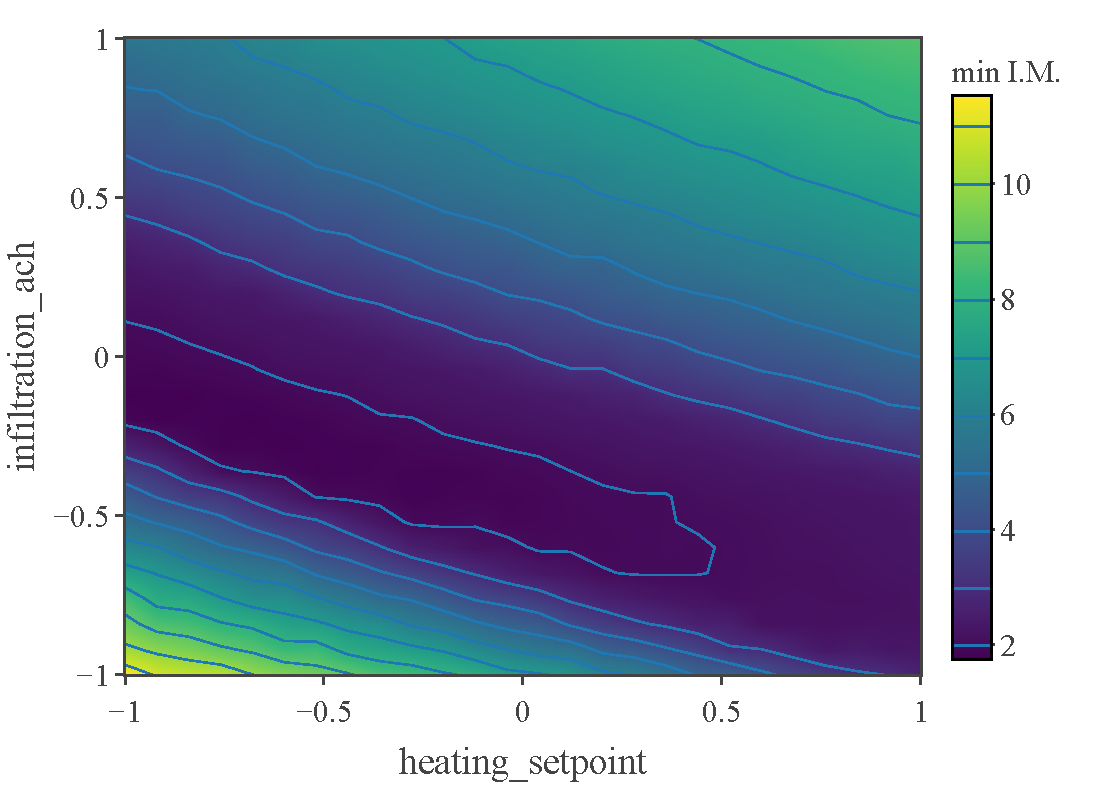
\includegraphics[width=\scale]{Gas_Compatibility/Min_Impl/minImpl_MD=20_x=1_y=6}
 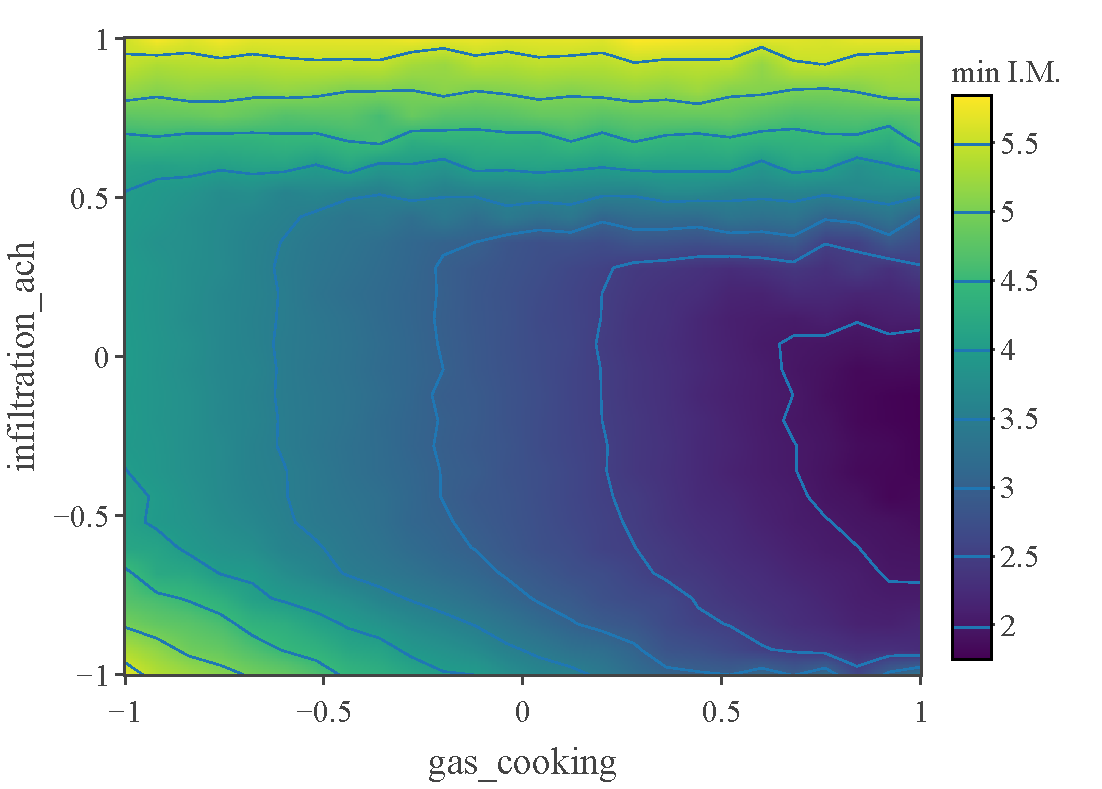
\includegraphics[width=\scale]{Gas_Compatibility/Min_Impl/minImpl_MD=20_x=8_y=6}\\
 \hspace{\scale}
  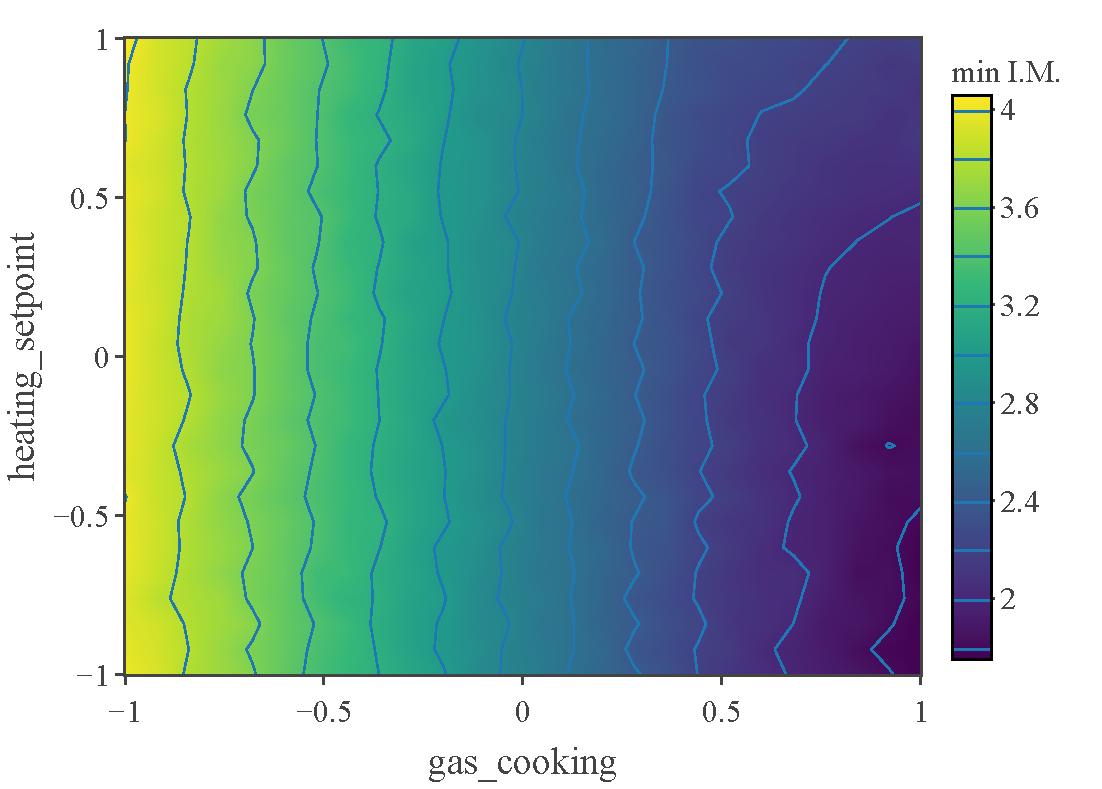
\includegraphics[width=\scale]{Gas_Compatibility/Min_Impl/minImpl_MD=20_x=8_y=1}
 \caption{20\% model discrepancy}
 \label{Fig_Min_Implaus_20MD}
\end{figure}

\begin{figure}
\centering
 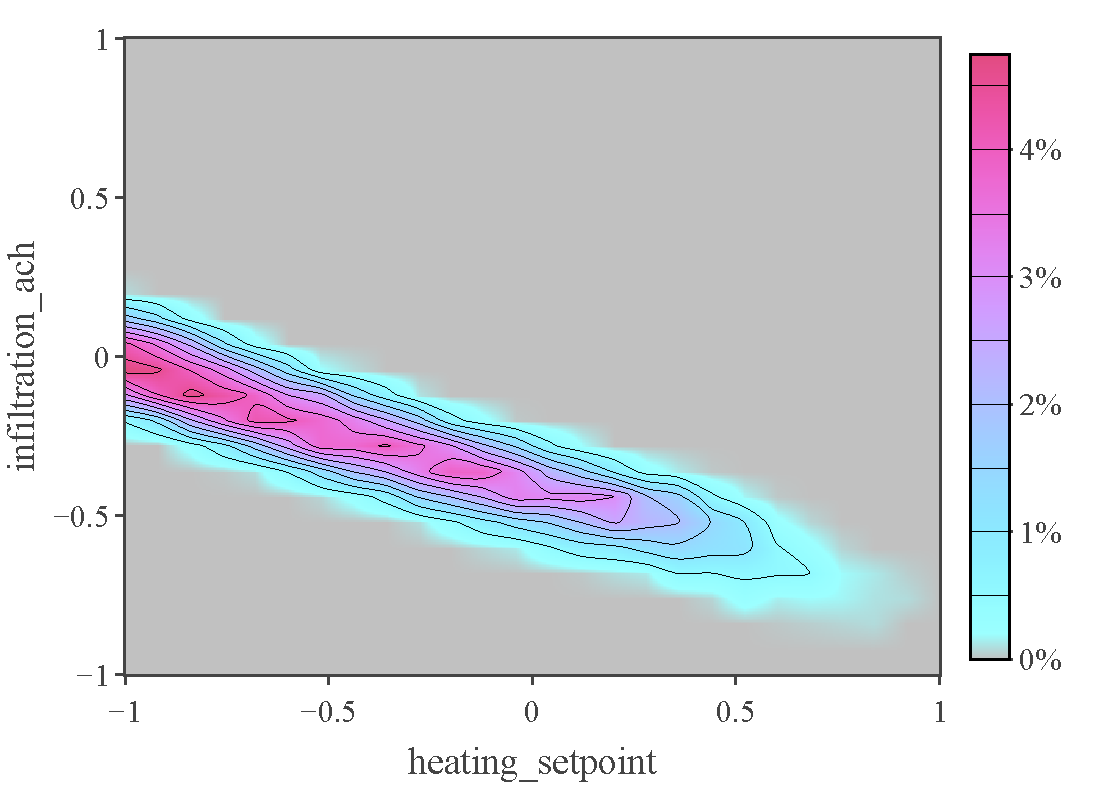
\includegraphics[width=\scale]{Gas_Compatibility/Opt_Depth/Depth_MD=10_x=1_y=6}
 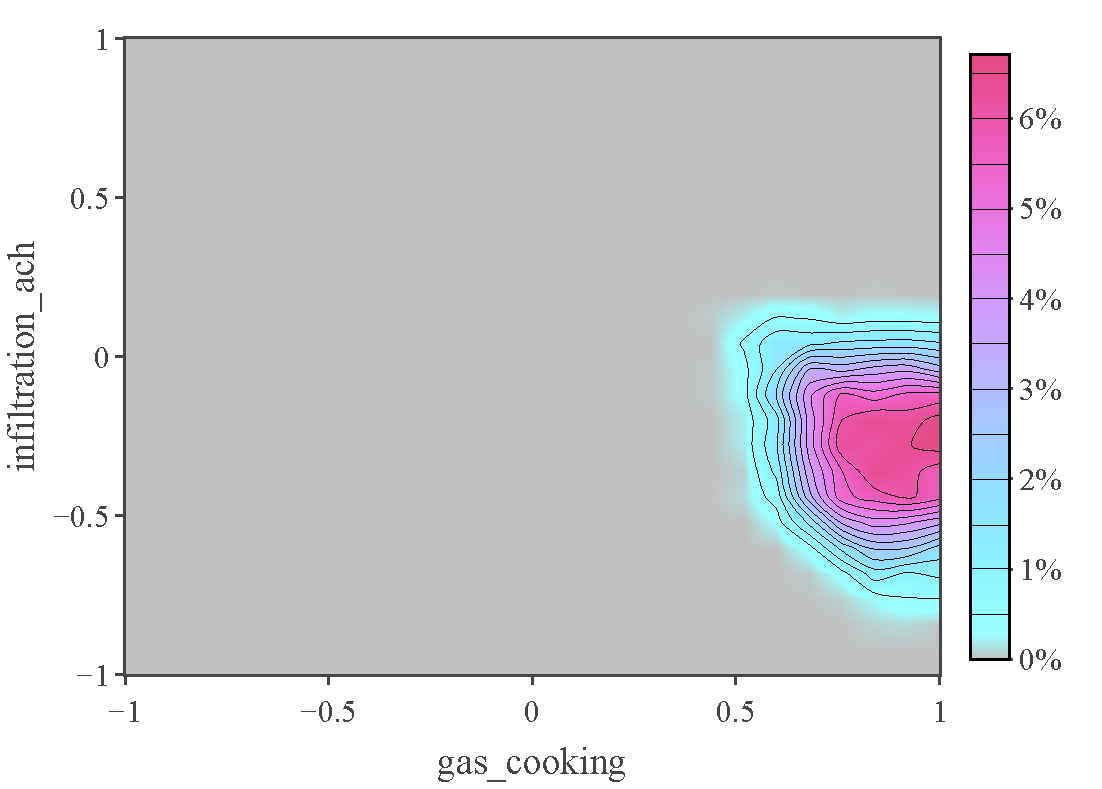
\includegraphics[width=\scale]{Gas_Compatibility/Opt_Depth/Depth_MD=10_x=8_y=6}\\
 \hspace{\scale}
  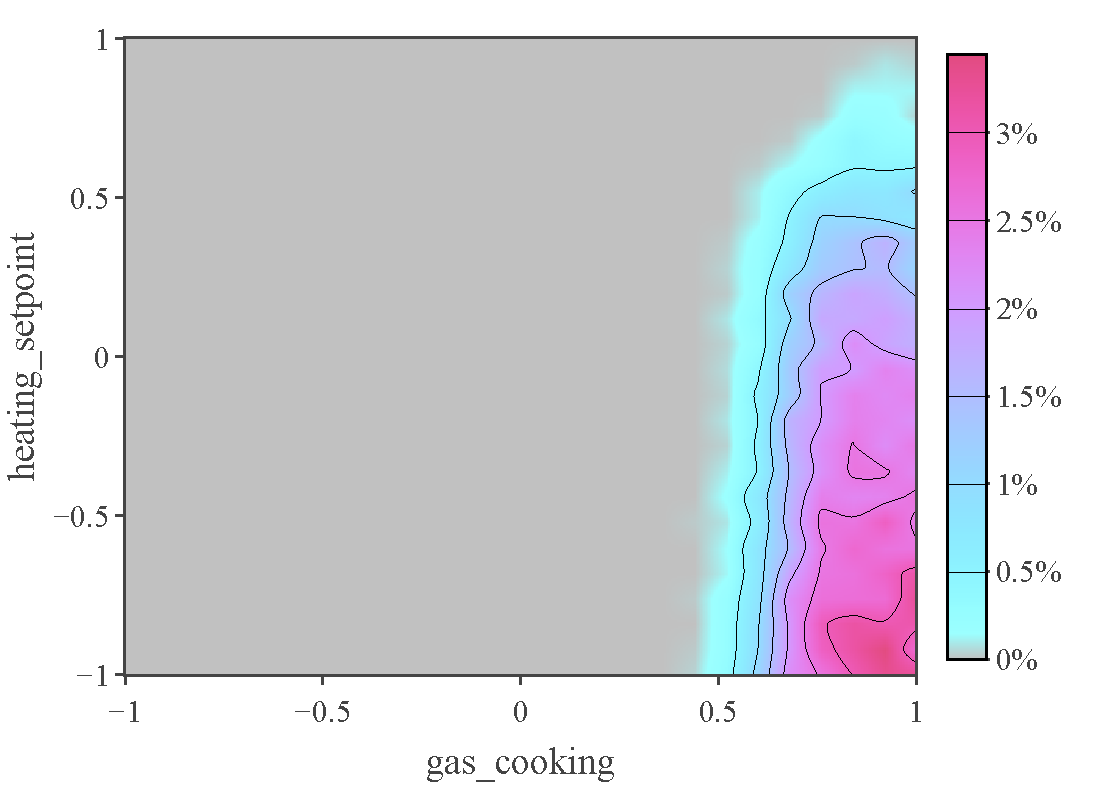
\includegraphics[width=\scale]{Gas_Compatibility/Opt_Depth/Depth_MD=10_x=8_y=1}
 \caption{}
 \label{Fig_Opt_Depth_10MD}
\end{figure}


\begin{figure}
\centering
 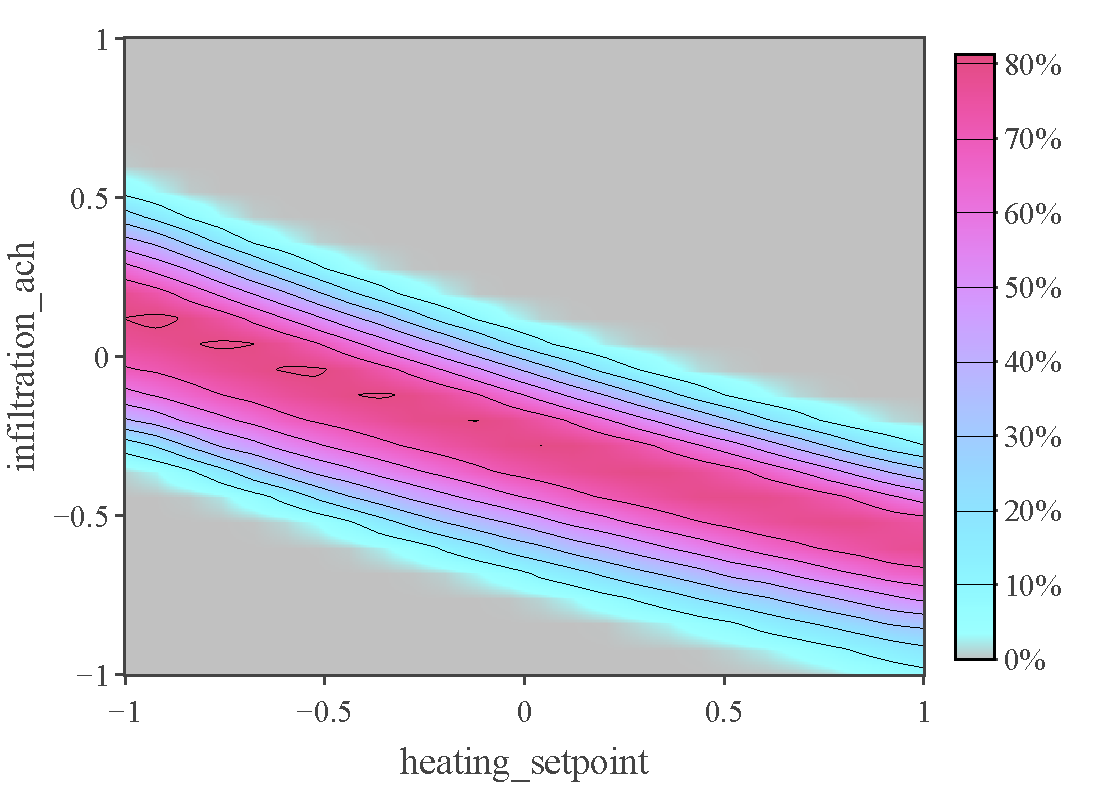
\includegraphics[width=\scale]{Gas_Compatibility/Opt_Depth/Depth_MD=20_x=1_y=6}
 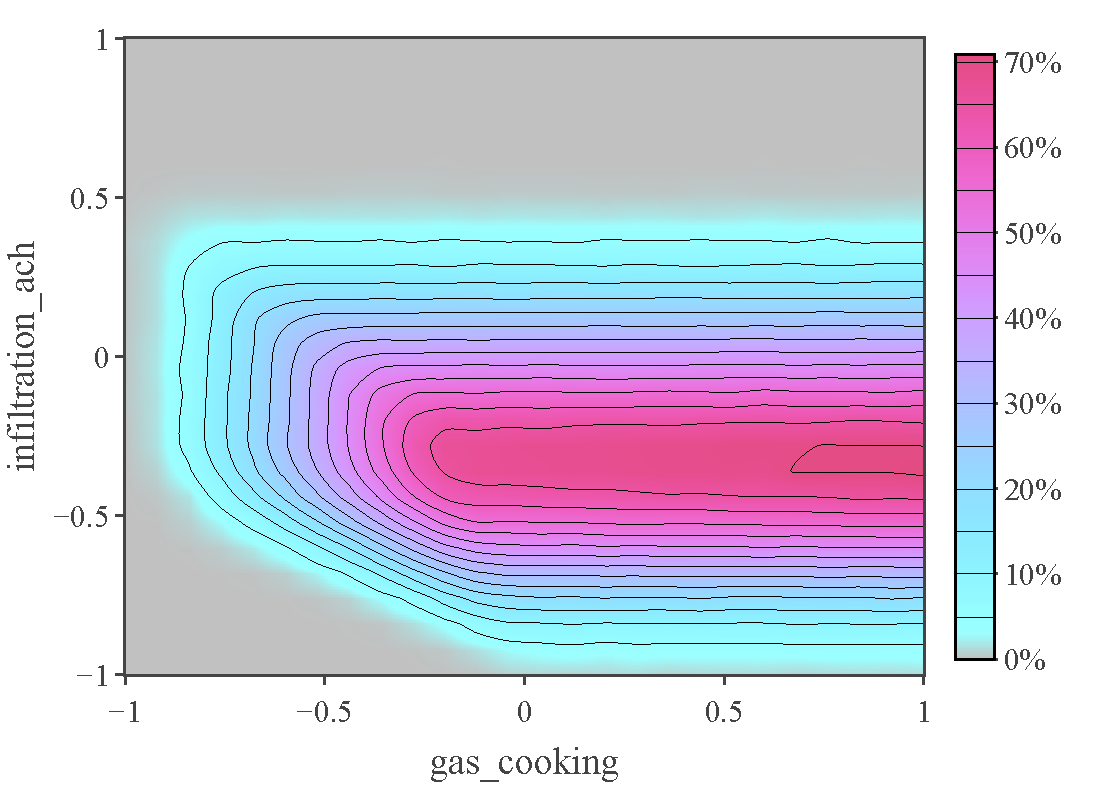
\includegraphics[width=\scale]{Gas_Compatibility/Opt_Depth/Depth_MD=20_x=8_y=6}\\
 \hspace{\scale}
 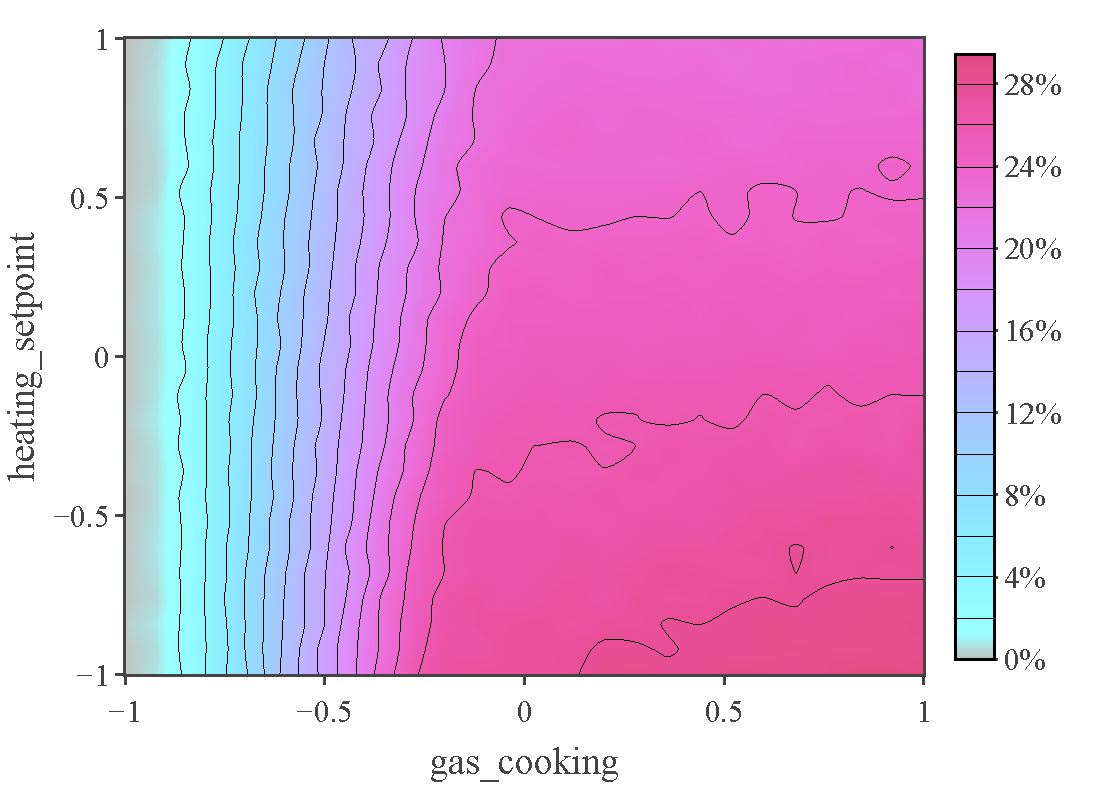
\includegraphics[width=\scale]{Gas_Compatibility/Opt_Depth/Depth_MD=20_x=8_y=1}
 \caption{}
 \label{Fig_Opt_Depth_20MD}
\end{figure}


In order to explore the compatibility between different regions of the space and the observed data, we generate a Sobol quasi-random sample of $N = 10^7$ points in the 8-dimensional cube $C={[-1,1]}^8$.


We start by examining the results when $T=4$.
In the case where only $5\%$ model discrepancy (MD) is considered, none of the 10 million points is classified as non-implausible according to condition~\eqref{Condition}. Further inspection also reveals that no point can be found which matches any eight of the nine months simultaneously.
However, by accounting for larger model discrepancy, non-implausible inputs can be found: they constitute $0.33\%$ of the space when $10\%$ MD is accounted for, and $19.5\%$ of the space when MD is increased to $20\%$.





In~\autoref{Table_Implausibility} we report these percentages, together with the percentages of space which are deemed non-implausible when compatibility with a single month is imposed. The percentages corresponding to the case $T=5$ are also shown. We see that the non-implausible fraction of space corresponding to a $5\%$ MD is essentially zero also in the $T=5$ case. If we accept that observed consumptions come with a measurement error of at most $5\%$, then this suggests that the discrepancy between the simulator and reality is likely to be higher than $5\%$.


As easily foreseeable from the plots of~\autoref{Fig_Output_Hist}, \autoref{Table_Implausibility} reveals that notable parts of the space result non-implausible when compared with the observation of a single month, although the insersection of these parts of the space may be (almost) empty, as in the two $5\%$ MD cases. With the exception of these two rows, however, we can notice the following: the fraction of non-implausible space is about 2 orders of magnitude higher than the product of non-implausible fractions with respect to the single months. This suggests indeed that the nine conditions imposed in equation~\eqref{Condition} are not independent of each other, but rather positively correlated.





























\end{document}
